%% LaTeX2e class for student theses
%% thesis.tex
%% 
%% Karlsruhe Institute of Technology
%% Institute for Program Structures and Data Organization
%% Chair for Software Design and Quality (SDQ)
%%
%% Dr.-Ing. Erik Burger
%% burger@kit.edu
%%
%% Version 1.3.2, 2017-08-01

%% Available page modes: oneside, twoside
%% Available languages: english, ngerman
%% Available modes: draft, final (see README)
\documentclass[twoside, english]{sdqthesis}
\usepackage{mathtools}
\usepackage{pgfplots}
\usepackage{tabularx}
\pgfplotsset
{
	compat                   = newest,
	every tick/.append style = thin,
	width= .95 \textwidth
}
% safe mode so we dont redefine \: etc
\usepackage[safe]{tipa}

%% ---------------------------------
%% | Information about the thesis  |
%% ---------------------------------

%% Name of the author
\author{Emanuel Jöbstl}

%% Title (and possibly subtitle) of the thesis
\title{Reverberation robust acoustic modelling using time delay neural networks}

%% Type of the thesis 
\thesistype{Master's Thesis}

%% Change the institute here, ``IPD'' is default
\myinstitute{Interactive Systems Lab}

%% You can put a logo in the ``logos'' directory and include it here
%% instead of the SDQ logo
% \grouplogo{myfile}
%% Alternatively, you can disable the group logo
% TODO: Put the CMU logo in the logos directory, remove nogrouplogo
\nogrouplogo

%% The reviewers are the professors that grade your thesis
\reviewerone{Prof. Prof. Dr. Alexander Waibel}
\reviewertwo{Prof. Dr.-Ing. Rainer Stiefelhagen}

%% The advisors are PhDs or Postdocs
\advisorone{M.Sc. Markus Müller}
%% The second advisor can be omitted
\advisortwo{Dr. Sebastian Stüker}

%% Please enter the start end end time of your thesis
\editingtime{4. November 2017}{3. May 2018}

\settitle

%% --------------------------------
%% | Settings for word separation |
%% --------------------------------

%% Describe separation hints here.
%% For more details, see 
%% http://en.wikibooks.org/wiki/LaTeX/Text_Formatting#Hyphenation
\hyphenation{
% me-ta-mo-del
}

%% --------------------------------
%% | Bibliography                 |
%% --------------------------------

%% Use biber instead of BibTeX, see README
\usepackage[citestyle=numeric,style=numeric,backend=biber]{biblatex}
\addbibresource{thesis.bib}

%% ====================================
%% ====================================
%% ||                                ||
%% || Beginning of the main document ||
%% ||                                ||
%% ====================================
%% ====================================
\begin{document}
\tikzset{%
	every neuron/.style={
		circle,
		draw,
		minimum size=1cm
	},	
	tdnn neuron/.style={
		rectangle,
		draw=black,
		fill=black!10,
		minimum height=0.5cm,
		minimum width=0.1cm 
	},
	neuron vmissing/.style={
		draw=none, 
		scale=4,
		text height=0.333cm,
		execute at begin node=\color{black}$\vdots$
	},
	neuron hmissing/.style={
		draw=none, 
		scale=2,
		text height=0.333cm,
		execute at begin node=\color{black}$\hdots$
	},
}

\tikzstyle{state}=[shape=circle,draw=black]
\tikzstyle{observation}=[shape=rectangle,draw=black]
\tikzstyle{lightedge}=[<-,dotted]
\tikzstyle{mainstate}=[state,thick]
\tikzstyle{mainedge}=[<-,thick]

\newcommand*\dif{\mathop{}\!\mathrm{d}}

\newcommand{\weightillustration}[3]{
\begin{minipage}{\linewidth}
	\centering
	\vspace{5mm}	
	\includegraphics[angle=90,width=0.9\linewidth]{#1}
	\captionof{figure}{#2}
	\label{#3}
\end{minipage}
}

\newcommand{\smallweightillustration}[3]{
	\begin{minipage}{\linewidth}
		\centering
		\vspace{5mm}	
		\includegraphics[angle=90,width=0.5\linewidth]{#1}
		\captionof{figure}{#2}
		\label{#3}
	\end{minipage}
}

%% Set PDF metadata
\setpdf

%% Set the title
\maketitle

%% The Preamble begins here
\frontmatter

%% LaTeX2e class for student theses: Declaration of independent work
%% sections/declaration.tex
%% 
%% Karlsruhe Institute of Technology
%% Institute for Program Structures and Data Organization
%% Chair for Software Design and Quality (SDQ)
%%
%% Dr.-Ing. Erik Burger
%% burger@kit.edu
%%
%% Version 1.3.2, 2017-08-01

\thispagestyle{empty}
\null\vfill
\noindent\hbox to \textwidth{\hrulefill} 
\iflanguage{english}{I declare that I have developed and written the enclosed
thesis completely by myself, and have not used sources or means without
declaration in the text.}%
{Ich versichere wahrheitsgemäß, die Arbeit
selbstständig angefertigt, alle benutzten Hilfsmittel vollständig und genau
angegeben und alles kenntlich gemacht zu haben, was aus Arbeiten anderer
unverändert oder mit Änderungen entnommen wurde.}
 
 
%% ---------------------------------------------
%% | Replace PLACE and DATE with actual values |
%% ---------------------------------------------
\textbf{Pittsburgh, 1st of Mai, 2018}
\vspace{1.5cm}
 
\dotfill\hspace*{8.0cm}\\
\hspace*{2cm}(\theauthor) 
\cleardoublepage

\setcounter{page}{1}
\pagenumbering{roman}

%% ----------------
%% |   Abstract   |
%% ----------------
 
%% For theses written in English, an abstract both in English
%% and German is mandatory.
%%
%% For theses written in German, a German abstract is sufficient.
%%
%% The text is included from the following files:
%% - sections/abstract

\includeabstract

%% ------------------------
%% |   Table of Contents  |
%% ------------------------
\tableofcontents

\listoffigures
\listoftables

%% -----------------
%% |   Main part   |
%% -----------------

\mainmatter

%%% LaTeX2e class for student theses
%% sections/content.tex
%% 
%% Karlsruhe Institute of Technology
%% Institute for Program Structures and Data Organization
%% Chair for Software Design and Quality (SDQ)
%%
%% Dr.-Ing. Erik Burger
%% burger@kit.edu
%%
%% Version 1.3.2, 2017-08-01

\chapter{Introduction}
\label{ch:Introduction}

Automated Speech Recognition is an important way of human computer interaction. The fundamental problem Automated Speech Recognition attempts to solve is to transform natural spoken language to text, which can then easily be processed by computer systems. Especially with the advent of smart mobile devices, more and more use cases for Automated Speech Recognition are available, mainly in the form of smart assistants as described in \cite{lopez2017alexa}. There are also many use cases which are not facing end users, for example the automated transcription of university lectures, as outlined in \cite{muller2016lecture}.

Despite the recent success of automated speech recognition, many systems still rely on microphones which are close to the speaker, or microphone arrays and beamforming. For many use cases, this is a serious draw back. Users might want to use their smart assistant without picking up their device every time. During lectures, it is hard to transcribe questions from the audience. 

\cite{yoshioka2012making} gives a good overview about the problems that arise when distant microphones are used. The most prominent problem is reverberation. Reverberation happens, informally speaking, when a signal is overlayed with weaker, delayed copies of itself. 

The goal of this work is to investiage how Automated Speech Recognition could be made more robust against reveberation. More specifically, a the focus is put on providing a more robust acoustic model using Time Delay Neural Networks. 

\section{Reveberation and reverbed Audio}

This section will focus on a formal definition of reverberation and provide some intuition why reveberation makes Automated Speech Recognition difficult. First, we give a very brief introduction to signal processing and system theory, according to the book \cite{leon2015signale}.

\subsection{Continous Signals and Systems}

An audio signal can, as any other continous \textit{signal}, be described as a continous function $y(t)$ where $t$ indicates the time. In literature, the argument $t$ is often dropped  when not explicitely needed to make equations easier to read.  
Signals can be fed into \textit{systems}, which in turn creates an output signal. In the context of this work, we only consider linear, time invariant systems. 
\\
Let $S$ be a linear time invariant system, $y_1$, $y_2$ continous signals, and $c_1$, $c_2$ constants. The following properties hold if and only if a given system is an linear time invariant system: 

\[S\{c_1 y_1(t) + c_2 y_2(t)\} = c_1 S\{y_1(t)\} + c_2 S\{y_2(t)\} \tag{linearity}\]

The linear property allows us to treat application of a system to a signal as a linear transformation in the function space our signals are defined in. 

\[y_1(t) = S\{y_2(t)\} \implies y_1(t - t0) = S\{y_2(t - t0)\} \tag{time invariance}\]

The time invariance propery guarantees that the behavior of a system never depends on the time. In other words, if the input signal to a system is shifted in time, the only difference to the output is a shift in time as well.

\[
\begin{rcases*}
y_1(t') = y_2(t') \\
x_1(t') = S\{y_1(t')\} \\ 
x_2(t') = S\{y_2(t')\} \\
\end{rcases*} \implies x_1(t') = x_2(t') \tag{causality}\]

The causality property guarantees that, if two signals are equal for all times $t'$ before a chosen time $t_0$, the output signals of the system processing this signals will also be equal up to this point. Simply put, the output of a system up to time $t_0$ can not depend on any input that happens after $t_0$. It is worth to note that all real systems are always causal. 
\\ \\
A linear time-invariant system can be characterized by its so called impulse response $g$, defined as the system output when presented with a so called dirac impulse $\delta$.

\[g(t) = S\{\delta(t)\}\]

The dirac impulse $\delta$ is a function that is formally defined by the following equation. 

\begin{align}
g(t_2) = \int_{-\infty}^{\infty} y(t)\delta(t - t_2) dt \label{eq:dirac} 
\end{align}

It can be said that the dirac impulse is zero for all $t$ not equal to zero. The integral over the dirac impulse defined to be one. 
\\ \\
Given definition \ref{eq:dirac}, as well as the linear property, we can show that the impulse response of a system is indeed sufficient to calculate the output signal for any given input signal. 
\begin{align*}
x(t) &= S\{y(t)\} \\
	 &= S\left\{\int_{-\infty}^{\infty} y(\tau)\delta(\tau - t) d\tau \right\} \\
	 &= \int_{-\infty}^{\infty} y(\tau)S\{\delta(\tau - t)\} d\tau \\
	 &= \int_{-\infty}^{\infty} y(\tau)g(\tau - t) d\tau
\end{align*}

Furthermore, we define the convolution operation, $*$, for two given signals as follows.

\[
 (y_1 * y_2)(t) = \int_{-\infty}^{\infty} y(\tau)y_2(\tau - t) d\tau \tag{(convolution)}
\]

A convolution is thus an operation that combines two functions to create a new function. Given this definition, we can write the output signal $x$ of a system $S$ given an input signal $y$ as convolution with the impulse response $g$ of the system. 

\[
x(t) = S\{y(t)\} = (y * g)(t)
\]

\subsection{Properties of Reverberation}

The acoustic properties of a room can be approximated as a linear time invariant system. The properties of this system are dependent on the properties of the room itself, for example the shape, size and surface of the wall, as well as the location of the sound source and the location of the receiver. Especially regarding automated speech recognition, \cite{ritter2016training} gives results that show that the location of a speaker relative to the microphone can have a very large impact on recognition results.

The measured impulse response of a real reveberation can be seen in figure \ref{fig:air_rir}. This specific sample is taken from the Aachen Impulse Response database \cite{jeub2009binaural}. Such a sample can be created by creating a very brief sound impulse, for example a clap, in an otherwise silent room, and then recording the sound for a few seconds. 

As described in \cite{yoshioka2012making}, we can divide the impulse response into the direct sound itself, early reflections, and late reverberation. The intuition behind is that the original sound wave arrives at the receiver first. After that, reflections of the signal which were reflected once by the walls of the room arrive. These reflections are already dampened significantly. Then, reflections of reflections will be received, and so on, until the sound waves become so weak that the room is silent again. 
\\ \\
\begin{minipage}{\linewidth}
	\makebox[\linewidth]{
		\begin{tikzpicture}
			\begin{axis}[ytick=\empty,height=6cm, ylabel=Amplitude, xlabel=Milliseconds, 
			xticklabel style={name=T\ticknum}]
			\addplot table [x expr=\coordindex / 4,y=amplitude,color=black,mark=none] {data/air0053bilecture};
			
			\end{axis}	
			\draw[] (1.2,4) -- (1,4) node[anchor=east,font=\tiny] {Sound};
			\draw[decorate, decoration={brace}] (1.3,3.2) -- (3.00,3.2) node[midway, anchor=south,font=\tiny] {Early Reflections};	
			\draw[decorate, decoration={brace}] (3.05,3.2) -- (11.8,3.2) node[midway, anchor=south,font=\tiny] {Late Reverberations};	
			\label{fig:air_rir}
		\end{tikzpicture}
	}
	\captionof{figure}{Room impulse response of a lecture hall}
\end{minipage}

It is important to note that late reveberations can be measureable for several hundred milliseconds.\\\\

To illustrate the impact of reflection and reveberation in a more formal way, we can use the decomposition into direct sound, early reflection, and late reverberation. We define a rather crude approximation of a room impulse response that subsequently overlays an audio signal with weaker copies of itself.

\[
g_{rir}(t) = w_0 \delta(t) + \sum_{1}^{n} w_n * delta(t - t_n)
\]

Here, $w_n$ are weighting factors, which represent the dampening of our reflections. $t_n$ are the delays until our reflection is received. We now consider the system $S_{rir}$ associated with the impulse response $g_{rir}$, apply the audio signal $y$ and observe the output $x$.

\begin{align*}
x(t) &= S_{rir}\{y(t)\} \\
     &= (g_{rir} * y)(t) \\
     &= \int_{-\infty}^{\infty} g(\tau)y(\tau - t) d\tau \\
     &= \int_{-\infty}^{\infty} \left[ w_0 \delta(t) + \sum_{n} w_n * \delta(t - t_n)\right] y(\tau - t) d\tau \\
     &= \int_{-\infty}^{\infty} \delta(t) y(\tau - t) d\tau + \sum_{n}  \int_{-\infty}^{\infty} w_n \delta(t - t_n) y(\tau - t) d\tau  \\
     &= w_0 y(t) + \sum_{n} w_n y(t - t_n)
\end{align*}

If the room impulse response is non-zero over at a certain time interval $t_n$, the audio signal produced at $t$ will still influence the received signal $x$ at $t + t_n$. 

\subsection{Impact of Reverberation on Digital Audio Samples}

Before formally introducing automated speech recognition during a later chapter, we want to show that the impact of reverberation can be significant for many applications that process sound or speech.\\ \\
Before a signal can be processed on a computer, it has to be measured. This process is called \textit{sampling}. Formally, we can describe sampling as the following operation, where $t_A$ is called the sampling interval. We call $y_{digital}$ a discrete signal. 

\[
y_{digital}(t) = y(t) * \sum_{n = 0}^{\infty} \delta{t - nt_A} 
\]

Since this yields a time series of inifinite length, signals are usually cut into pieces, which are then independently processed from each other. This is called windowing. For the most simple form of windowing, we can set all signal values outside of a certain range to be zero. Formally, this can be defined by multiplying the signal with a rectangle function $\sigma_{rect,a}(t)$ .

\[
\sigma_{rect,a}(t) = \begin{cases}
1 &,-a < t < a \\
0
\end{cases}
\]

When working with signals, especially for classification tasks, methods built upon the \textit{fourier transform} are used very often. The fourier transform transforms a signal $y(t)$ from its time domain to the frequency domain $Y(f)$. The resulting function $Y(f)$ is called the spectrum and gives the distribution of energy over all frequencies for the original signal $y(t)$. The fourier transformation can be defined for continous or descrete signals, as well as for descrete and windowed signals. In the case of descrete and windowed signal, this is called the \textit{short time fourier transform}, which was first described in \cite{gabor1946theory}. It can formally be defined as follows, with an arbritary window function $\sigma$:

\[
Y(n, \omega) = \sum_{m = -\infty}^{\infty} y(mt_A) \sigma((n - m)t_A) e^{-j \omega n}  
\]

The function $Y(n, \omega)$ gives the energy for a certain time window $n$ and a frequency window $\omega$. The time resolution depends reciprocally on the frequency resolution and vice versa. It is not possible to increase the frequency resolution while not decreasing the time resolution.\\ \\

We can investigate the effects of a reverbed signal on the short time fourier transform by applying the same approach as in the previous chapter. The resulting short time fourier spectrum of the reverbed and sampled signal is given as follows.

\begin{align*}
Y(n, \omega) = \sum_{m = -\infty}^{\infty} w_0 y(mt_A) \sigma((n - m)t_A) e^{-j \omega n} + 
\sum_{m = -\infty}^{\infty} \sum_{n} w_n y(mt_A - t_n) \sigma((n - m)t_A) e^{-j \omega n}  
\label{eq:stftnoise}
\end{align*}

Equation \ref{eq:stftnoise} shows that, for large $t_n$ and $w_n$, significant noise is added to neighboring time windows. To recapitulate from the last chapter, the $t_n$ for a large room can be up to several tenths of seconds, while the window size for most applications is in the hundrets of milliseconds. 
\\ \\
This mathematic observation shall serve as a motivation for this work. Reverberation, especially late reverberation can be a hard problem that significantly distorts measurements of signals. We conclude the introduction with 

\begin{minipage}{\linewidth}
	\makebox[\linewidth]{
		\begin{tikzpicture}
		\begin{axis}[xlabel=Time, ylabel=Frequency, ytick=\empty, width= .50\textwidth]
		\addplot [] 
		graphics[xmin=0,xmax=3,ymin=0,ymax=1] {images/abc_spectrogram.png};
		\end{axis}
		\end{tikzpicture}
		\begin{tikzpicture}
		\begin{axis}[xlabel=Time, ylabel=\empty, ytick=\empty, width= .50\textwidth]
		\addplot [] 
		graphics[xmin=0,xmax=3,ymin=0,ymax=1] {images/abc_noise_spectrogram.png};
		\end{axis}
		\end{tikzpicture}
	}
	\captionof{figure}{Room impulse response of a lecture hall}
\end{minipage}

TODO: Nice picture of noisy STFT







\section{Related Work}
\label{ch:related_work}
This chapter will enumerate related work on acoustic modelling using TDNNs. 

\chapter{Related Work}
\label{ch:realted_work}

This chapter will give a brief introduction to neural networks and time delay neural networks, as well as an introduction automated speech recognition with hidden markov models. These are the necessary building blocks for the work presented in this thesis. At the end of this chapter, we will also briefly present research that directly inspired this work. 

\section{Neural Networks}
\label{sec:neural_networks}

In machine learning research, the goal of a \textit{neural network} is to approximate arbitrary functions. The basic idea of neural networks, so called \textit{perceptrons}, were first introduced by Rosenblatt in \cite{rosenblatt1958perceptron}. While the first neural networks were biologically motivated, neural networks can be interpreted as composition of functions. The relation between these functions forms a directed graph. In this work, we will only cover \textit{feed forward neural networks}. They are called feed forward neural networks because there are no feedback connections: The relation between all functions in the neural network forms an acyclic directed graph. Feed forward networks are an important building block for many machine learning applications. 
\\
More formally, as described in \cite{Goodfellow-et-al-2016}, a feed forward neural network can be described as a model $y = f^*(x, \theta)$, approximating an existing function $y = f(x)$. In this example $x$ is the input, $y$ is the output and $\theta$ are the model parameters which are learned during training. $f$ is the function to approximate and $f^*$ is a composition of many functions with the parameters $\theta$. 
\\
In practice, the functions composing a feed forward neural network are often simply chained, so that their relation graph simply forms a path. In this case, the functional components are called layers. A feed forward neural network of this form with $n$ layers can be written as follows:

\[
y = f^*_n \dots (f^*_2(f^*_1(x, \theta_1), \theta_2) \dots, \theta_n)
\]

For this type of neural network, $f^*_1$ is applied to the input, then $f^*_2$ is applied to the output of $f^*_1$, until the final layer is reached. The output of the final layer is the output of the neural network. Figure \ref{fig:simple_feed_forward_nn} shows a graph based representation of such a neural network. Each node represents a function, arrows represent data flows. 

\begin{minipage}{\linewidth}
	\makebox[\linewidth]{
	\begin{tikzpicture}[x=1.5cm, y=1.5cm, >=stealth]
	
	\node [every neuron] (n0) at (0*1-1,2.5-0) {$x$}; 
	\node [every neuron] (n1) at (1*1-1,2.5-0) {$f^*_1$}; 
	\node [every neuron] (n2) at (2*1-1,2.5-0) {$f^*_2$}; 
	\node [neuron hmissing] (n3) at (3*1-1,2.5-0) {}; 
	\node [every neuron] (n4) at (4*1-1,2.5-0) {$f^*_n$}; 
	\node [every neuron] (n5) at (5*1-1,2.5-0) {$y$}; 
	
	\draw [->] (n0) -- (n1);
	\draw [->] (n1) -- (n2);
	\draw [->] (n2) -- (n3);
	\draw [->] (n3) -- (n4);
	\draw [->] (n4) -- (n5);
	
	\end{tikzpicture}
	}
	\captionof{figure}{Simple graphical interpretation of feed forward neural network}
	\label{fig:simple_feed_forward_nn}
	\hspace{1cm}
\end{minipage}


Even with this simplification, it has been shown that such a feed forward neural network can approximate any function with any desired accuracy. This is called the \textit{universal approximation theorem}, the proof can be found in \cite{hornik1989multilayer}. The caveat is finding the correct function $f^*_n$ to use in each layer and the correct parameters $\theta_n$. Also, finding the function to approximate is non-trivial in the first place. We will discuss these problems in the next sections. 

\subsection{Training Neural Networks}

As with most machine learning approaches, we train the neural  network using by using a \textit{training dataset}, containing a lot of data points sampled from the distribution we seek to approximate. We usually do not want the neural network to excel on the training data set, but rather to perform well on unseen data. This ability is called \textit{generalization}. We can approximate the error on unseen data by testing the neural network on a \textit{test dataset}. The test dataset must never be used for adjusting the neural network parameters, as this will make the test dataset worthless. The situation where a network performs well on the training dataset but worse on the test dataset is called \textit{overfitting}. The network basically memorizes the distribution of the training dataset, but fails to generalize on the test dataset. \\
Given the definition in the past section, we can treat the problem of training a given neural network as finding appropriate parameters $\theta$ to minimize a certain \textit{error function} or \textit{loss function} $E = \mathcal{L}(y)$, where $E$ denotes the error and $y$ the network output. The error $E$ is usually some metric that judges the network performance based on the training data set. The state of the art algorithm for optimizing the parameters of a neural network is called \textit{stochastic gradient descend}, a special application of naive \textit{gradient descend}.
\subsubsection{Naive Gradient Descent}
\label{sec:gradient_descend}
To apply gradient descend, we have to calculate the derivative of the loss function, given a certain input, with respect to a certain parameter $\theta_i$. Since this derivative is multi-dimensional, it is called the \textit{gradient}. Given a feed forward neural network, we can write the error as follows:

\[
E = \mathcal{L}(f^*_n \dots (f^*_2(f^*_1(x, \theta_1), \theta_2) \dots, \theta_n))
\]

Thus, the derivative of the error with respect to a certain weight can be calculated by applying the chain rule.  

\[
\frac{\delta E}{\delta \theta_i} = 
	\frac{\delta \mathcal{L}}{\delta y_n}
	\frac{\delta f^*_n}{\delta y_{n - 1}}
	\dots
	\frac{\delta f^*_{i + 2}}{\delta y_i}
	\frac{\delta f^*_i}{\delta \theta_i}
\]

Where $y_k$ is the result of $f^*_k$. \\
We know that the gradient $\frac{\delta E}{\delta \theta_i}$ will become zero in a local minimum, local maximum or saddle point of our error $E$. Since the gradient also gives the direction of the steepest slope, we can simply update our parameters iteratively, until we converge into a local minimum.

\[
	\theta_{i, t+1} = \theta_{i, t} - \epsilon * \frac{\delta E_{t}}{\delta \theta_{i, t}}
\]

In this equation, $t$ denotes the current time and the parameter $\epsilon$ is the so-called learning rate. $\epsilon$ has to be chosen by the designer of the neural network and influences not only the speed of convergence, but also whether the network converges at all. In literature, propagating the error gradient through a neural network is called \textit{backpropagation}. Backpropagation in the context of neural networks was first described in \cite{werbos1974beyond}.

\subsubsection{Stochastic Gradient Descend}

In practice, naive gradient descend does not work well, as described in \cite{wilson2003general}. The reason is that the function we seek to optimize when training a neural network is not convex and might have many local minima. Optimizing iteratively on a stationary error term makes this approach prone to falling into local minima. \\ \\
The state of the art algorithm for training neural networks is called \textit{stochastic gradient descent} (\textit{SGD}), which was first described in a context of neural networks in \cite{bottou1991stochastic}. Stochastic gradient descent introduces two fundamental changes and is. First, we no longer calculate our error term and corresponding gradient for the whole dataset, but for a randomly sampled subset of our data set, which is called a \textit{mini batch}, where the size of the mini batches is a design parameter. Second, we decrease our learning rate while training progresses. According to \cite{Goodfellow-et-al-2016}, iterating on mini batches adds noise to our error term, which in turn offers a regularization effect which was shown to lead to better generalization.
\\ \\
The noise introduced by stochastic gradient descend originates from the fact that we batch our dataset. Even if all batches, if averaged, represent the same distribution as our whole test dataset, each batch has a slightly different distribution. The shape of the loss function, and thus the gradient, changes slightly with each mini batch. This is the main reason why stochastic gradient descend is less prone to get stuck in local minima then naive gradient descend. The noise added by this stochastic process does not go away, even when we reach a global minimum. According to \cite{Goodfellow-et-al-2016}, this is be the main motivation for decreasing the learning rate over time. Furthermore, this property implies that the mini batch size is also an important design choice for achieving good generalization, not only for achieving fast training. 
\\ \\
A disadvantage of stochastic gradient descend is the slower convergence, since we need more steps. This is remedied by the fact that it is easier to calculate the gradient for a small mini batch instead of the whole dataset at once. In practice, we usually shuffle our dataset, split it into mini-batches, and then process each mini batch once. An iteration over all mini batches in the dataset is called an \textit{epoch}. 

\subsubsection{Learning Rates and Learning Rate Scheduling}

With stochastic gradient descend, we choose a separate learning rate $\epsilon_k$ for each epoch $k$. In the scope of this work, we only introduce \textit{exponential decay}, a very simple scheduling algorithm for the learning rate, although numerous other schedulers exist. \\
Exponential starts with a learning rate $k_0$ for the initial batch and multiplies the learning rate by a factor of $0 < p < 1$ after each epoch. 
\[
k_n = k_{n - 1} * p
\]
A variant of exponential decay keeps the learning rate constant for a number epochs, until the improvement of error measured on the test dataset falls below a certain threshold $t$. This variant is called \textit{newbob}. Newbob scheduling is widely used by the speech recognition community. It was first introduced in \cite{berkely2000newbob}.

\subsubsection{Momentum}

\textit{Momentum} is another technique that was shown to avoid local minima. When using momentum, we do not apply the gradient directly to our model, but rather use a linear combination of the gradient of the last batches. There are multiple versions to achieve momentum when using stochastic gradient descend. This work uses the notation introduced in \ref{polyak1964some} and throughly analyzed in the context of deep learning in \ref{sutskever2013importance}:
\begin{align*}
\upsilon_{i, t+1} &= \upsilon_{i, t} * \rho + \epsilon * \frac{\delta E_{t}}{\delta \theta_{i, t}} \\
\theta_{i, t+1} &= \theta_{i, t} - \upsilon_{i, t+1}
\end{align*}
Here, $\upsilon$ is called the \textit{velocity}, it is a linear combination of the last velocity and the current gradient. $\rho$ is the term defining the momentum. It defines how much of the velocity is added to the current gradient. All other variables are defined as in section \ref{sec:gradient_descend}.

\subsection{Neural Network Architectures}

In practice, neural network layers are often formed by combining an affine transformation with a non-linear function. Since affine transformations of data vectors can be interpreted as matrix-vector multiplications, we can write a layer function in the following way, where $x_k$ is the input vector for $k$th layer, $W_k$ is the matrix defining the affine transformation of the $k$th layer, and $\varphi$ is a non-linear activation function of layer $k$.
\[
f^*_k(x_k) = \varphi_k(W_k x_k)  
\]
The count of layers, as well as the size of each $W_k$ are design decisions and depend on the task. We call the count of layers \textit{depth} of a neural network, and count of rows in $W_k$ the \textit{width} of layer $k$. The contents of $W_k$, called the \textit{weights} of layer $k$, are the trainable parameters $\theta$ for models of this form.
\pagebreak
\subsubsection{Activation Functions}

Non-linear activation functions, or simply \textit{activation functions}, can be roughly classified into two groups: Activation functions which are applied element-wise and thus do not change the dimension of the data, as well as activation functions which are applied on groups of elements of the input vector and change the dimension. The latter case is commonly fund with so called pooling functions. The choice of the activation function $\varphi$ has significant impact on the performance of a neural network and has been subject to many bodies of research, as summarized in \cite{thoma2017analysis}. In this work, we will only discuss the \textit{ReLU}, \textit{p-norm} and \textit{softmax} activation functions. 

\subsubsection*{Rectified Linear Unit (ReLU)}
% ReLU
\begin{minipage}{0.45\textwidth}
	\[\varphi^{ReLU}(x) = \begin{cases}
	0 & x < 0 \\
	x & x \geq 0
	\end{cases}\]
	First introduced in \cite{krizhevsky2012imagenet}, ReLU nonlinearities have proven successful in practice. The computation of ReLU nonlinearity is cheap, also the gradient never saturates for positive values of $x$. For negative values, the gradient is zero, which can be a disadvantage.  
\end{minipage}
\hfill
\begin{minipage}{0.45\textwidth}
\begin{tikzpicture}[baseline=(current bounding box)]
\begin{axis}[xmin=-2,xmax=2,ymin=-2,ymax=2,axis lines = middle,xlabel = $x$,ylabel = $\varphi^{ReLu}(x)$,clip = false]
\addplot+[mark=none,blue,domain=-2:0] {0};
\addplot+[mark=none,blue,domain=0:2] {x};
\end{axis}
\end{tikzpicture} 
\captionof{figure}{The ReLU function.}
\end{minipage}
% L2 Pooling

\subsubsection*{P-norm}
\begin{minipage}{0.45\textwidth}
	\[\varphi^{Lp}(X) = \sqrt[p]{ \sum_{x \in X}{x^p} } \] 
	The p-norm nonlinearity was described by \cite{zhang2014improving}. This nonlinearity operates on a set $X$ of input elements and reduces them to one. The group size as well as the $p$ are a design parameter. For a fixed $p$ of $2$, the p-norm is also called \text{L2 pooling}.
\end{minipage}
\hfill
\begin{minipage}{0.45\textwidth}
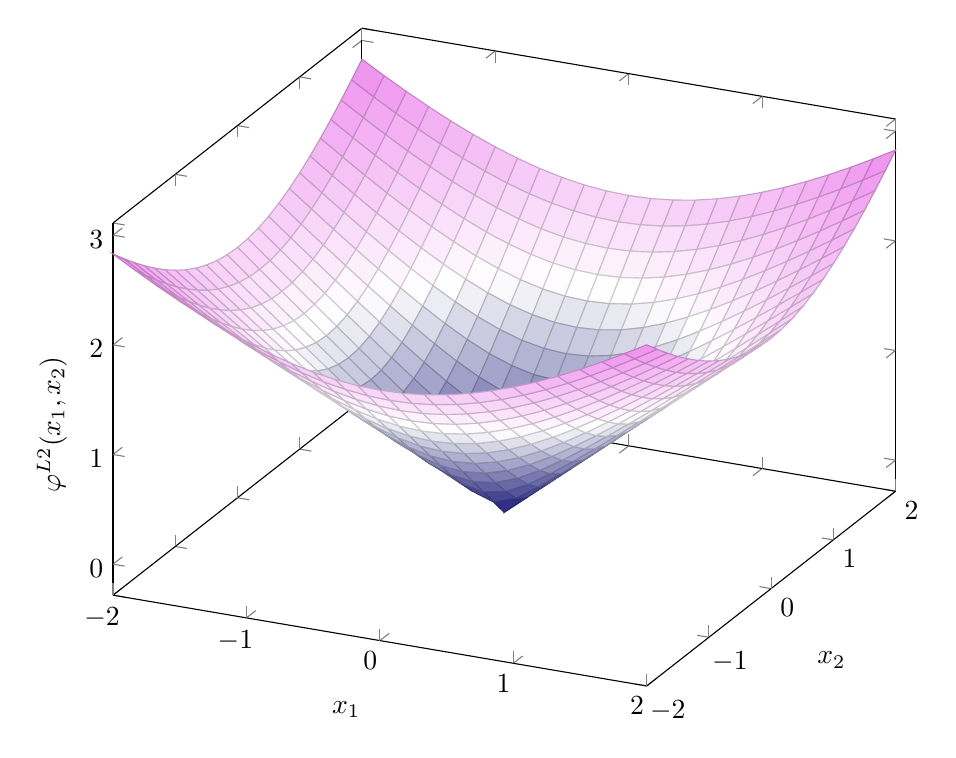
\begin{tikzpicture}[baseline=(current bounding box)]
\begin{axis}[xmin=-2,xmax=2,ymin=-2,ymax=2,xlabel = $x_1$,ylabel = $x_2$,zlabel = $\varphi^{L2}({x_1, x_2})$,colormap/violet,clip = false]
\addplot3[surf,samples=25, domain=-2:2]
{sqrt(x * x + y * y)};
\end{axis}
\end{tikzpicture}
\captionof{figure}{Example of p-norm with $p = 2$ and and an input group containing two values}
\end{minipage}

\subsubsection*{Softmax}
\begin{minipage}{0.45\textwidth}
	\[\varphi^{softmax}_{\tau}(X)_i = \frac{e^\frac{x_i}{\tau}}{ \sum_{x_j \in X} e^\frac{x_j}{\tau} } \]
	The softmax activation is defined as an operation over the whole input, but does not reduce the dimension. It maps all output values to a space between $0$ and $1$, preserves the rank of each output and also guarantees that the sum over all outputs is exactly $1$. Therefore it produces a valid probability distribution and is usually used for the last layer of a neural network for classification problems. The term $\tau$ is called the softmax temperature. It can be used to change the contrast of the distribution produced by the softmax activation. A higher temperature $\tau$ will lead to a distribution more smooth. A lower $\tau$ will lead to a more sharp distribution, that concentrates a higher probability at the maximum value. 
\end{minipage}
\hfill
\begin{minipage}{0.45\textwidth}
	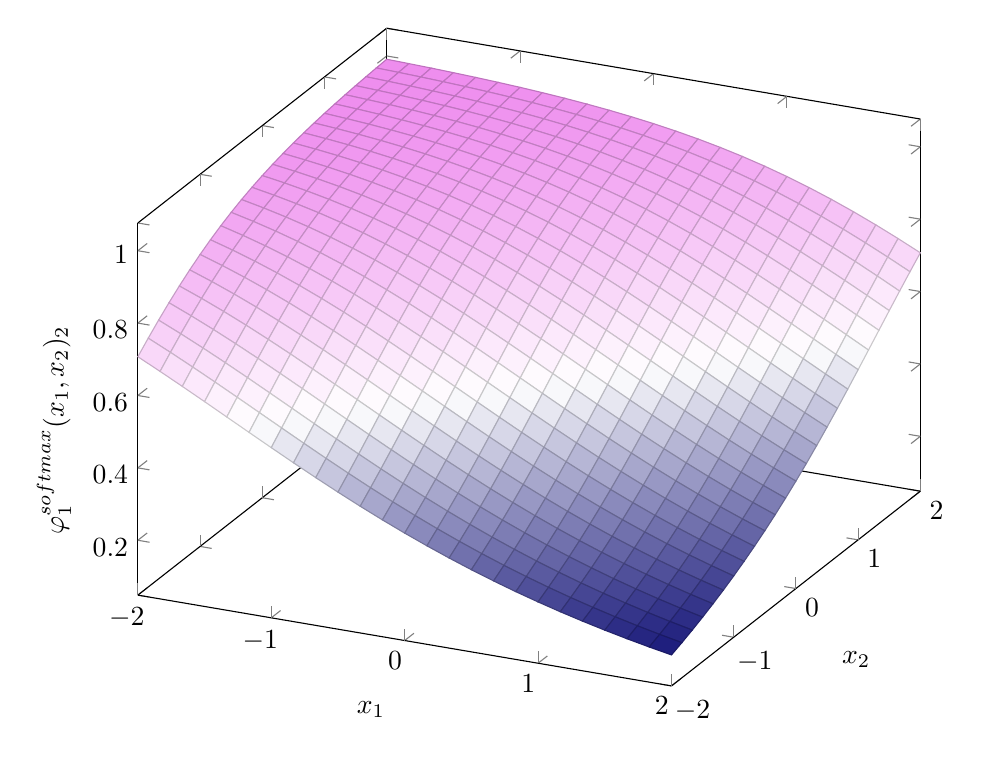
\begin{tikzpicture}[baseline=(current bounding box)]
	\begin{axis}[xmin=-2,xmax=2,ymin=-2,ymax=2,xlabel = $x_1$,ylabel = $x_2$,zlabel = $\varphi^{softmax}_{1}({x_1, x_2})_2$,colormap/violet,clip = false]
	\addplot3[surf,samples=25, domain=-2:2]
	{sqrt(e^y / (e^x + e^y) )};
	\end{axis}
	\end{tikzpicture}
	\captionof{figure}{Example of a vanilla softmax ($\tau = 1$) for an input vector containing two values}
	\vspace{0.5cm}
	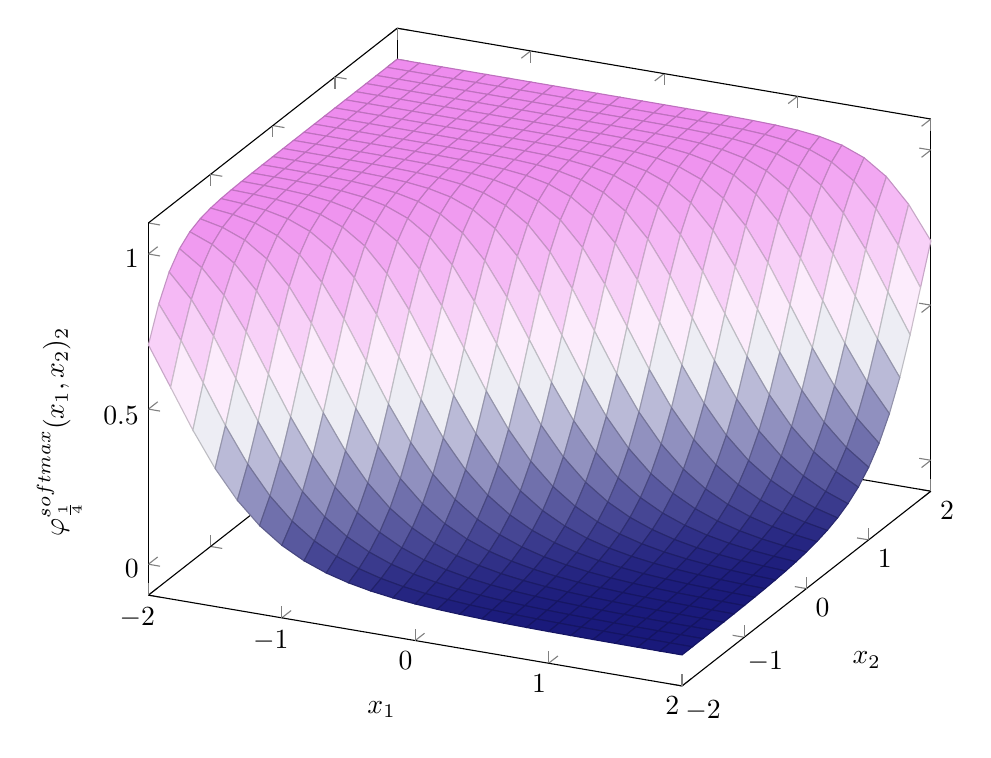
\begin{tikzpicture}[baseline=(current bounding box)]
	\begin{axis}[xmin=-2,xmax=2,ymin=-2,ymax=2,xlabel = $x_1$,ylabel = $x_2$,zlabel = $\varphi^{softmax}_{\frac{1}{4}}({x_1, x_2})_2$,colormap/violet,clip = false]
	\addplot3[surf,samples=25, domain=-2:2]
	{sqrt(e^(y * 4) / (e^(x * 4) + e^(y * 4)) )};
	\end{axis}
	\end{tikzpicture}
	\captionof{figure}{Example of a softmax with adjusted temperature ($\tau = \frac{1}{4}$) for an input vector containing two values}
\end{minipage}

\subsection{The Cross Entropy Loss Function}

There exist numerous loss functions for neural networks. Technically, any metric can be used as loss function, although loss functions do not necessarily have to be metrics. One of the most widely loss functions for classification tasks is the \textit{cross entropy} (\textit{CE}) function. For two  probability vectors $p$ and $q$, the cross entropy can be written as follows:

\begin{align}
H(p, q) = - \sum_{x} p(x) \log q(x)
\label{eq:cross_entropy_loss}
\end{align}

The cross entropy loss function has several important properties. First, it minimizes the so called \textit{Kullback-Leibler} (\textit{KL}) divergence. The Kullback-Leibler divergence measures the distance of two probability distributions and was introduced in \cite{kullback1951information}. The Kullback-Leibler divergence is equal to zero if, and only if, the two given distributions are also equal. For two probability vectors $p$ and $q$, it can be written in the following way:

\[
D_{KL}(p, q) = -\sum_{x} p(x) \log \frac{p(x)}{q(x)}
\]

To show the connection between the cross entropy and the Kullback-Leibler divergence, we first assume that $q$ is the distribution we seek to optimize. Thus $p$ can be thought of as an example from our training dataset, or in other words, the distribution we seek to match. Therefore, $p$, can be assumed to be constant. We can write the Kullback-Leibler divergence as follows: 

\begin{align*}
D_{KL}(p, q) &= - \sum_{x} p(x) \left[ \log p(x) - \log q(x) \right] \\
& = - \sum_{x} p(x) \log p(x) -\sum_{x} p(x) \log q(x)
\end{align*}

Since we are not interested minimizing the distribution $p$, we can drop the first sum, and thus receive the cross entropy loss as in equation \ref{eq:cross_entropy_loss}. \\ \\
When training neural networks, we often deal with classification problems. In this case, we seek to assign a single class to a given input sample, our target probability $p$ has exactly one element which is one, all other elements are zero. In this case, the cross entropy loss can be simplified to the so called \textit{negative log likelihood loss}, where $i$ is the index of the correct class in $p$. 

\[
D_{NLLL}(i, q) = -\log q(i)
\]

It has to be noted that this loss functions all operate on probability vectors: All elements have to be between $0$ and $1$ and sum to unity. Therefore, a softmax activation function is usually applied before calculating the loss. 

TODO: Section about picking data, and tips like like data augmentation? 

\section{Time Delay Neural Networks}

\textit{Time delay neural networks} were introduced by Waibel et. al in \cite{waibel1990phoneme}. The purpose time delay neural networks is to model long time dependencies in a robust way. The central idea behind this network type is to use several time frames of input, and to not use fully-connected layers, but rather layers that impose temporal structure. \\ \\
To achieve this, the network not only receives the current frame $x_{0,t}$ as input, but also the $n$ previous frames $x_{0,t - 1}, ..., x_{0,t - n}$ as input. These frames are delayed in time, hence the name. Then, the a weighted sum is applied to the input, where the weights are learned parameters. This is called a \textit{TDNN unit} or \textit{TDNN layer}. TDNN layers can be stacked. If this is the case, preceding layers have to be extended to produce an output that contains multiple time frames. \\
Formally, we can write for $x_{k,t}$, the output of the $k$-th TDNN layer at time t for the feature vectors with size one:
\[
x_{k,t} = \sum_{i = 1}^n w_{k, i} x_{k - 1, t - i}
\]
Where $w_{k, i}$ is denotes the $i$-th weight of the weighted sum used by the $k$-th layer. \\
This equation can be rewritten using a discrete convolution operator. In this case $w_k$ is called a convolution kernel. 
\[
x_{k} = w_{k} * x_{k - 1}
\]
For feature vectors containing more than one feature, we introduce the concept of \textit{channels}. A channel can be considered a dimension in the feature. We can write this case for $p$ input channels and $q$ output channels, where $w_{k, j}$ is now a multi-dimensional kernel, producing the output channel $j$. Each TDNN layer will learn $q$ such kernels, while each kernel is large enough to take all $p$ input channels into account. 
\[
x_{k,j} = w_{k, j} * x_{k - 1}
\]
The concept of interpreting TDNN layers as convolutions is not new, but very useful. The generalization to multi-dimensional convolutions is called \textit{convolutional neural networks} and was shown to be incredibly successful \cite{krizhevsky2012imagenet}. Since TDNNs only apply the convolution over the time dimensions, it can be useful to interpret a TDNN as a so called \textit{finite impulse response} (\textit{FIR}) filter. As described in \cite{leon2015signale}, finite impulse response filters are inherently stable, as they the output is always a sum of finite elements. They also do not accumulate rounding errors. \\
In \cite{waibel1990phoneme}, another interesting property is given: Since there are a lot less learned parameters than operations, a TDNN layer is forced to only focus on the most important features in the data, which leads to better generalization. This so-called \textit{parameter sharing} is achieved by averaging gradients of all operations for their respective weight, independently of the time context $t$. According to \cite{Goodfellow-et-al-2016}, this is one of the main reasons of success for convolutional neural networks in general. 

\subsection{Pooling, Stride and Splicing}

It should be noted that most successful convolutional architectures, as \cite{krizhevsky2012imagenet}, combine convolutional layers with pooling nonlinearities. This is done because pooling over the layer output enables to network to learn several different representations of the same concept, where the pooling will forward the most dominant to the next layer. \\
Furthermore, it was shown that using larger steps in the convolution operation can lead to better results \textit{springenberg2014striving}. In the context of TDNNs, this means that we would not use adjacent frames for concatenating our input, but frames which are further apart. In literature, this is called \textit{stride} or \textit{strided convolution}, where the the stride $s$ gives the distance between concatenated frame. For a strided convolution, the input vector can be written as:
\[
x_{0,t}, x_{0,t + s}, ..., x_{0,t + ns}
\] 
It is also possible to define a list of indexes $S = (s_1, ..., s_n)$ to concatenate, which is especially useful if the distance between concatenated frames should not be uniform. This operation is called \textit{splicing} and was introduced by \cite{peddinti2015jhu}. In this case, our input vector becomes: 
\[
x_{0,ts_1}, x_{0,t + s_2}, ..., x_{0,t + s_n}
\] 

\section{Automated Speech Recognition}
\label{ch:HMM_ASR}
\textit{Automated speech recognition} (\textit{ASR}) is the task of generating a text transcription from a given sample of spoken language using a computer system. In literature, this problem is also referred to as \textit{speech to text} (\textit{SST}). \\
Many approaches exist for solving this task. In this work, we will focus on automated speech recognition using systems that are based on hidden markov models for modeling language. The contents of this this section, except otherwise noted, is based upon the lecture Automated Speech Recognition of Karlsruhe Institute of Technology \cite{kitasr2018stueker}, which is in turn based on the books \cite{schukat1995automatische} and \cite{huang2001spoken}. \\ \\
Automated speech recognition systems built on hidden markov models usually follows an architecture that separates \textit{preprocessing} of the audio signal and \textit{decoding}. The preprocessing transforms a brief time window of the audio signal into a feature vector. The decoding uses a statistical model assembled from an \textit{acoustic model}, a \textit{dictionary} and a \textit{language model} to calculate the most likely text representation, given the feature vectors.\\ \\

More formally, we can treat the decoding as a classification problem. Let $a$ be a set of feature vectors, we seek to find the word sequence $w^*$ that was most likely for $a$ under our model. That can formally be written as follows, where $p(w|a)$ is the conditional probability of event $w$ given $a$:

\[
w^* = \underset{w}{\arg \max} \; P(w|a)
\] 
We do not know $P(w|a)$, but can re-write it using Bayes' theorem:

\[
w^* = \underset{w}{\arg \max} \; \frac{P(a|w) P(w)}{P(a)}
\]

Since $p(a)$ is the same for all possible word sequences $w$, we can drop the denominator from this equation:

\begin{align}
w^* = \underset{w}{\arg \max} \; P(a|w) P(w)
\label{eq:asr_base_formula}
\end{align}

Equation \ref{eq:asr_base_formula} is called the \textit{fundamental equation of automated speech recognition}. While the fundamental equation seems straight forward, the difficult task is to create a reliable and computationally tractable model for approximating the probability of an acoustic feature given a word sequence, $p(a|w)$ and the probability of observing a word sequence $p(w)$. For this task, \textit{hidden markov models} built from the acoustic model, language model and dictionary are used. We will first describe the preprocessing, then briefly introduce hidden markov models, then introduce the three components and then show how they are combined into a single model, which is then used by the decoder. 

\subsection{Preprocessing}
Preprocessing transforms some audio signal into a sequence of feature vectors. To do so, we sample an audio signal using a microphone, then the signal is windowed and the spectrum is calculated for each window of the signal. This process is called short time fourier transform, as defined in the introduction in equation \ref{eq:stft}. Hence, the resulting spectral coefficients are also often called \textit{fourier coefficients}. It should be noted that there are more sophisticated approaches, notably the \textit{continous wavelet transform}, as described in \cite{mallat1999wavelet}, which has better properties in terms of time and frequency resolution. \\ \\
There exist numerous approaches to transform the spectrum of a signal to useful features. In this work, we only discuss so called \textit{log-mel coefficients}. 
\subsubsection{Log-Mel Coefficients}
Log-mel coefficients were introduced in \cite{waibel1990phoneme} and \cite{waibel1983comparative}. This approach is physiologically motivated. To be specific, the mel-scale provides a better relative frequency resolution in lower frequencies. \\
As given in \cite{poser1990speech}, the mel-scale is defined by the following relation to the regular frequency spectrum in Hertz: 
\[
MEL(f)=2595\log _{10}\left(1+{\frac {f}{700}}\right)
\]
Very often, the number of coefficients is reduced to get smaller feature vectors $(\sigma_1, ..., \sigma_n)$. This is done by summing all coefficients in certain windows $\sigma_k$ on the mel-scale: 
\[
MEL_k = \int \sigma_k(f) * MEL(f) \delta f 
\]

In practice, a triangle window is often used. In literature, the weighted sum is also referred to as \textit{filter bank} \cite{zhan1997vocal}. \\
The $k$-th log-mel coefficient is then calculated by applying a logarithm:
\[
lMEL_k = \log(MEL_k) 
\]
\\ \\
In literature, \textit{Mel-Frequency-Cepstral-Coefficients} (\textit{MFCCs}) are often mentioned. They are not to be confused with log-mel coefficients. MFCCs can be calculated by applying an inverse discrete cosine transform on the the log-mel coefficients.

% Our experiments use VTLN with a warp factor of 1.0. According to the janus implementation, that does not do anything. 
%\subsubsection{Vocal Tract Length Normalization}
%TODO: 
%https://www.lti.cs.cmu.edu/sites/default/files/CMU-LTI-97-150-T.pdf

\subsection{Hidden Markov Models}
To explain hidden markov models, we first introduce the concept of a \textit{markov chain}. A markov chain is a sequence of random variables $X = x_1, x_2, \dots. x_{t - 1}, x_{t} \dots, x_T$ and a finite number of states $s_1, \dots, s_n$, where the probability of each entering a certain state at time $t + 1$ at only depends on the state at time $t$:

\[
P(x_{t + 1} = s_{j_{t + 1}} | x_{t} = s_{j_t}, x_{t - 1} = s_{j_{t - 1}} \dots, x_{1} = s_{j_{1}}) = P(x_{t + 1} = s_{j_{t + 1}} | x_{t} = s_{j_t})
\] 

This assumption is also called the \textit{markov assumption}. If the probability of moving from state $s_{j_t}$ to state $s_{j_{t + 1}}$ is independent of the current time $t$, we call a markov chain \textit{homogeneous}. \\ \\
We now extend our homogeneous markov chain and assume that we can no longer observe the state $s_{j_t}$ at a given time $t$ directly, but a symbol $v_k$ that was emitted. We formally define: 
\begin{align*}
S &= \{s_1, \dots, s_n\} \tag{states} \\
V &= \{v_1, \dots, v_m\} \tag{symbols} \\
A &= (a_{ij}) \tag{state tansmission probability} \\
a_{ij} &= p(x_{t+1} = s_j | x_{t} = s_i) \\
B(k) &= (b_j(k)) \tag{emisson probability} \\
b_j(k) &= p(v_k | x_t = s_j) \\
\pi &= (\pi_i) \tag{initial state probability} \\
\pi_i &= p(x_1 = s_i)
\end{align*}

The tuple $\lambda = (S, V, A, B, \pi)$ specifies a \textit{hidden markov model}. We furthermore introduce the graphical notation for hidden markov models seen in figure \ref{fig:hmm}. Unspecified transitions and observations have probability zero. 

\begin{minipage}{\linewidth}
	\makebox[\linewidth]{
		\begin{tikzpicture}[x=1.5cm, y=1.5cm, >=stealth]
		
		\node[state] (s1) at (0,2) {$s_1$}
		edge [loop above] node[above] {$a_{11}$} ();
		\node[state] (s2) at (3,2) {$s_2$}
		edge [<-,bend right=45] node[auto,swap] {$a_{12}$} (s1)
		edge [->,bend left=45] node[auto,swap] {$a_{21}$} (s1)
		edge [loop above] node[above] {$a_{22}$} ();
		\node[state] (s3) at (6,2) {$s_3$}
		edge [<-,bend right=45] node[auto,swap] {$a_{23}$} (s2)
		edge [->,bend left=45] node[auto,swap] {$a_{32}$} (s2)
		edge [loop above] node[above] {$a_{33}$} ();
		% observations
		\node[observation] (v1) at (1.5,0) {$v_1$}
		edge [lightedge] node[auto] {$b_1(1)$} (s1)
		edge [lightedge] node[auto,swap] {$b_2(1)$} (s2);
		\node[observation] (v2) at (4.5,0) {$v_2$}
		edge [lightedge] node[auto] {$b_2(2)$} (s2)
		edge [lightedge] node[auto,swap] {$b_3(2)$} (s3);
		\end{tikzpicture}
	}
	\captionof{figure}{Graphical example of a hidden markov model with three states and two observations}
	\label{fig:hmm}
	\hspace{1cm}
\end{minipage}

\subsubsection{Forward and Backward algorithm}
Given a sequence of observed emissions, a so called observation $O = \{o_1, \dots, o_t\}$, a hidden markov model can be used to evaluate the probability of the observation, given the parameters $p(O, \lambda)$. For calculating this joint probability, the \textit{forward algorithm} or the \textit{backward algorithm} can be used used. For the forward algorithm, let $\alpha_T(j)$ be the probability of having observed $O$ and being in state $s_j$ at the end of the observation. We define recursively for any previous time $t$:
\begin{align*}
\alpha_1(j) &= \pi_j b_j(o_1) \\
\alpha_t(j) &= b_j \sum_{i = 1}^{N} a_{ij}\alpha_{t-1}(i) \\
p(O|\lambda) &= \sum_{j = 1}^{N} \alpha_T(j)
\end{align*}
For the backward algorithm, we define a similar recursive algorithm, starting from the latest time observation. Here, $\beta_0(j)$ is the probability of observing $O$ when starting from state $s_j$.
\begin{align*}
\beta_T(j) &= 1 \\
\beta_t(j) &= \sum_{i = 1}^{N} a_{ij}b_j(o_{t+1}) \beta_{t+1}(i) \\
p(O|\lambda) &= \sum_{j = 1}^{N} \beta_0(j)
\end{align*}
\subsubsection{Decoding Problem}
Besides calculating the probability of an observation sequence, finding the most likely state sequence $X = \{X_1, X_2, \dots, X_T\}$ given an observation $O$ and a hidden markov model $\lambda$ is also of interest. 
This problem is called the \textit{decoding problem}, which is solved by the \textit{viterbi algorithm}. In the scope of this work, a formal definition of the viterbi algorithm is not necessary. 

\subsubsection{Learning Hidden Markov Model Parameters}
Given a hidden markov model topology, which is essentially only the number of states $n$ and the number of emission symbols $m$, as well as a training set of observations $O$, we can use the so called \textit{Baum-Welch} algorithm to optimize the initial state probabilities $\pi$, transmission probabilities $A$ and emission probabilities $B$. \\ \\
We first define two auxiliary variables, given an observation $O$ and the parameters $\lambda$: $\gamma_t(i)$, the probability of being in state $i$ at time $t$ and $\xi_t(i, j)$, the probability of being $i$ at time $t$ and state $j$ at time $t + 1$.

\begin{minipage}{0.45\textwidth}
\begin{align*}
\gamma_t(i) &= P(x_t = i|O,\lambda) \\
&= \frac{P(x_t = i, O|\lambda)}{P(O|\lambda)} \\
&=\frac{\alpha_t(i)\beta_t(i)}{\sum_{j = 1}^{N} \alpha_t(j) \beta_t(j)} 
\end{align*}
\end{minipage}
\hfill
\begin{minipage}{0.45\textwidth}
\begin{align*}
\xi_t(i, j) &= P(x_t = i,x_{t + 1} = j|O,\lambda) \\
&= \frac{P(x_t = i,x_{t + 1} = j, O|\lambda)}{P(O|\lambda)} \\
&=\frac{\alpha_t(i)a_{ij}\beta_{t + 1}(j)b_j(o_{t + 1})}{\sum_{i = 1}^{N} \sum_{j = 1}^{N} \alpha_t(i)a_{ij}\beta_{t + 1}(j)b_j(o_{t + 1})}
\end{align*}
\end{minipage}

Using this two auxiliary variables, we can find new parameters $\lambda$ iteratively. Let $\pi^*$, $A^*$ and $B^*$ be the new parameters after one iteration of the Baum-Welch algorithm. 

\begin{align*}
b^*_j(k) &= \frac{\sum_{t = 1, o_t = v_k}^{T} \gamma_t(j)}{\sum_{t = 1}^{T} \gamma_t(j)} \\
\pi^*_i &= \gamma_1(i) \\
a_{ij}^*  &= \frac{\sum_{t = 1}^{T} \xi_t(i, j)}{\sum_{t = 1}^{T} \gamma_t(j)} 
\end{align*}

It should be noted that the Baum-Welch algorithm is a special case of the \textit{expected maximization} {\textit{EM}} algorithm applied to hidden markov models. The expected maximization algorithm gives a maximum-likelihood estimate of parameters, even if the data set used for the estimation has incomplete or missing values. A proof can be found in \cite{bilmes1998gentle}. 

\subsection{Acoustic Model}
\label{sec:acoustic_model}
Before we explain the purpose of the acoustic model, we have to introduce the linguistic concepts of \textit{phonemes}, \textit{phones} and \textit{allophones}. Phonemes are sound atoms in a spoken language, that are relevant for the meaning of a spoken word. In other words, if a phoneme in a spoken word changes, the meaning of this word would change. Allophones are different pronunciation version of the same phoneme. \textit{Phones} are simply distinct sounds that are found in a language, regardless of whether swapping a phone changes the meaning of the word or not. \\ \\
The acoustic model $A$ is responsible of giving us the probability of observing a certain feature $o$, for a given phone $\wp$. 
\[
	A_\wp(o) = p(o|\wp)
\]
Traditional acoustic models use classification schemes on feature vectors from the preprocessing. The most prominent technique here are gaussian mixture models, which combine several normal distributions to approximate a more complex distribution. The parameters of the acoustic model are usually learned using the Baum-Welch equations introduced in the previous section. \\ \\
Acoustic models might be extended to classifying allophones, or even include context dependencies on neighboring phones. Antother approach would be to model the start, middle, and end part of an phone as three distinct hidden markov model states, which represent the phone together. This has the advantage of introducing some speed invariance into the model: It does no longer matter whether a certain phoneme was spoken very slowly or fast. Figure \ref{fig:sub_three_allophone} shows a hidden markov model for such an approach. 

\begin{minipage}{\linewidth}
	\makebox[\linewidth]{
		\begin{tikzpicture}[x=1.5cm, y=1.5cm, >=stealth]
		
		\node[state] (s1) at (0,1) {$a_s$}
		edge [loop above] ();
		\node[state] (s2) at (3,1) {$a_m$}
		edge [<-,bend right=45] (s1)
		edge [loop above] ();
		\node[state] (s3) at (6,1) {$a_e$}
		edge [<-,bend right=45] (s2)
		edge [loop above] ();
		% observations
		\node[observation] (v1) at (0,0) {$a_s$}
		edge [lightedge] (s1);
		\node[observation] (v2) at (3,0) {$a_m$}
		edge [lightedge] (s2);	
		\node[observation] (v3) at (6,0) {$a_e$}
		edge [lightedge] (s3);
		
		\end{tikzpicture}
	}
	\captionof{figure}{Hidden markov model for an allophone model with three sub-states for start $a_s$, middle $a_m$ and end $a_e$}
	\label{fig:sub_three_allophone}
	\hspace{1cm}
\end{minipage}

\subsection{Dictionary}
\label{sec:dictionary}
The purpose of the dictionary is to describe the pronunciation of words in terms of phones. The dictionary is usually given. A common way to create a dictionary is to generate it using a set of rules and a list of words, and then fine-tune it by hand. The dictionary also contains different pronunciation variants for each word. 

\begin{minipage}{\linewidth}
	\makebox[\linewidth]{
		\begin{tikzpicture}[x=1.5cm, y=1.5cm, >=stealth]
		
		\node[state] (AX) at (0,0) {\textscripta };
		\node[state] (EH) at (0,1) {\textipa{E}};
		\node[state] (IX) at (0,2) {\textbari };
		
		\node[state] (N) at (1,1) {\textipa{n}}
		edge [<-,bend right=15] (AX)
		edge [<-] (EH)
		edge [<-,bend right=-15] (IX);
		\node[state] (EY) at (2,1) {\textipa{e}\textsci }
		edge [<-,bend right=45] (N);
		\node[state] (B) at (3,1) {\textipa{b}}
		edge [<-,bend right=45] (EY);
		
		\node[state] (AX2) at (4,1) {\textscripta }
		edge [<-,bend right=45] (B);
		\node[state] (L) at (5,1) {\textipa{l}}
		edge [<-,bend right=-45] (B)
		edge [<-,bend right=45] (AX2);
		\node[state] (AXR) at (6,1) {\textrhookschwa }
		edge [<-,bend right=45] (L);
		\end{tikzpicture}
	}
	\captionof{figure}{Markov chain for pronunciation variants of the word \textit{enabler}, where the state names correspond to their respective IPA phones}
	\label{fig:dictionary_hmm}
	\hspace{1cm}
\end{minipage}
Figure \ref{fig:dictionary_hmm} shows such a model for a single word. Emissions are not shown, as each state in this model refers the hidden markov model associated with the corresponding phoneme. Transitions that are not modeled in the dictionary are constant zero. 
 
\subsection{Language Model}
\label{sec:language_model}
The language model models the probability of word sequences, or in other terms, the probability of a word following a certain other world. Since languages tend to have many words, calculating the transmission probability for each given word pair would be intractable. Instead of this, so called $n$-gram language models are used. $n$-gram language models count the occurrence of word tuples of length $n$ in a large text corpora. The occurrences are then used to calculate the probability of a word $w_1$, given $n - 1$ predecessors $w_2, ..., w_n$.

\[
L(w_1) = P(w_1|w_2,...,w_n)
\]

For a $2$-gram model, the transition probabilities can be directly derived by norming the count of occurrences for each successor. An example for such a model is shown in figure \ref{fig:lm_hmm}. For larger $n$, we have to have a state for each feasible combination of words, which quickly becomes intractable. 

\begin{minipage}{\linewidth}
	\makebox[\linewidth]{
		\begin{tikzpicture}[x=1.5cm, y=1.5cm, >=stealth]
		
		\node[state,minimum size=1cm] (that) at (2,0) {that}
		edge [loop below] node[auto] {$\frac{1}{2}$} ();
		\node[state,minimum size=1cm] (is) at (0,3) {is}
		edge [<-,bend right=15] node[auto, swap] {$\frac{1}{4}$} (that)
		edge [->,bend right=-15] node[auto] {$\frac{1}{4}$} (that)
		edge [loop above] node[auto] {$\frac{1}{4}$} ();
		\node[state,minimum size=1cm] (not) at (4,3) {not}
		edge [<-,bend right=-15] node[auto] {$0$} (that)
		edge [<-,bend right=15] node[auto,swap] {$\frac{1}{2}$} (is)
		edge [->,bend right=15] node[auto, swap] {$0$} (that)
		edge [->,bend right=-15] node[auto] {$1$} (is)
		edge [loop above] node[auto] {$0$} ();
		\end{tikzpicture}
	}
	\captionof{figure}{Markov chain built from a $2$-gram language model for the sentence \textit{``That that is, is; that that is not, is not."}, omitting start and end literals}
	\label{fig:lm_hmm}
	\hspace{1cm}
\end{minipage}


\subsection{Decoding Process}

The decoding step combines the acoustic model, dictionary, and language model are combined into one large model to find the text for a given observed utterance. This section describes decoding in a very fundamental way. In real-world applications, may more details are considered.  \cite{huang2001spoken} gives a very detailed description of different decoding approaches.\\
It is possible decompose any word $w_i$ to a possible sequences of phones $(\wp_1, ..., \wp_n)$, using the dictionary. We can re-write the fundamental formula of speech recognition in the following way, using the language and acoustic model:
\begin{align*}
W^* &= \underset{W}{\arg \max} \; P(X|W) P(W) \\
&= \underset{W}{\arg \max} \; \left( \sum_{w_i \in W} \sum_{\wp_i \in w_i} A_{\wp_i}(o_i) \right) \sum_{w_i \in W} L(w_i)
\end{align*}
Here, $X = (o_1, ..., o_n)$ is an observation sequence, and $W = (w_1, ..., w_n)$ is a word sequence. \\ \\ 
We can also interpret the combination of the acoustic model, language model and dictionary as one large hidden markov model. With this interpretation, we can find the optimal solution $W^*$ with a search through the hidden markov model. We can do so by using a greedy breath-first search with a heuristic, that picks the next state to visit. Such a search algorithm is also called \textit{A* algorithm} in literature \cite{hart1968formal}. However, this approach is not tractable in practice, as the model becomes very large. Therefore, a so-called \textit{beam search} is used. A beam search simply discards paths with a probability that fall below a certain threshold, which we call $mb$. \\ \\
For a real-world implementation we consider three more details. First, we want to avoid multiplications, because they are computationally expensive. We therefore maximize the negative log-likelihood instead of raw probabilities. Second, we add the scaling factor $lz$ to weight the acoustic model versus the language model, which was shown to be very useful in practice. Also we add another parameter $lp$ which can be used to penalize too short or too long word sequences. 
\begin{align*}
W^* &= \underset{W}{\arg \max} \; -\log\left(P(X|W) P(W)^{lz} |W|^{lp} \right) \\
&= \underset{W}{\arg \max} \; -\log P(X|W) - lz\log P(W) -lp\log(|W|) 
\end{align*}

The master beam $mb$, and the coefficients $lz$ and $lp$ are hyper-parameters that have to be tuned for optimal results. 

\subsubsection{Draft}

This chapter will be focused on how ASR is done with Janus. It will contain: 
\begin{itemize}
	\item A brief introduction to HMM models
	\item A brief introduction to HMM-based ASR tools:
	\begin{itemize}
		\item description of n-gram language models, dictionaries and context-dependent phone models
		\item description of the purpose of an acoustic model
		\item explanation, about how the this component are combined to form a speech recognizer 
		\item example, showing how the language and phone models, as well as the dictionary are combined to form a HMM
	\end{itemize}
	\item A description of the Word-Error-Rate and Frame-Error-Rate metric. 
	\item An explanation about training HMM-based systems using the expected maximisation algorithm. 
\end{itemize}

\subsection{Time Delay Neural Networks}
\label{ch:TDNN}
The goal of this chaper is to provide a short introduction to neural networks, 
as well as explain the concept of TDNNs. It will contain:
\begin{itemize}
	\item A brief intro to MLPs and SGD
	\item Parameter coupling (convolutional neural networks)
	\item Time delay neural networks
	\item Interpretation of TDNNs as FIR filters
\end{itemize}

\subsection{Acoustic Modelling using Neural Networks}
\label{ch:acoustic_modelling}
The goal of this chapter is to describe the approach of using DNNs for acoustic modelling.
The contents will be: 
\begin{itemize}
	\item definition of the acoustic model training as a deep learning problem
	\item different discriminative training strategies
	\begin{itemize}
		\item Binary Cross Entropy loss on existing labels
		\item Bianry Cross Entropy with re-generating the labels, then trianing again
		\item Minimum Bayes Risk and variants, especially State-Minimum-Bayes-Risk
	\end{itemize}
	\item A brief section about common tricks used when trianing DNN acoustic models, 
	especially Exponential Decay/Newbob.
	\item If there is time left: A brief analysis of the 2nd derivative of the loss function
	during gradient descend.
\end{itemize}

\begin{minipage}{\linewidth}
	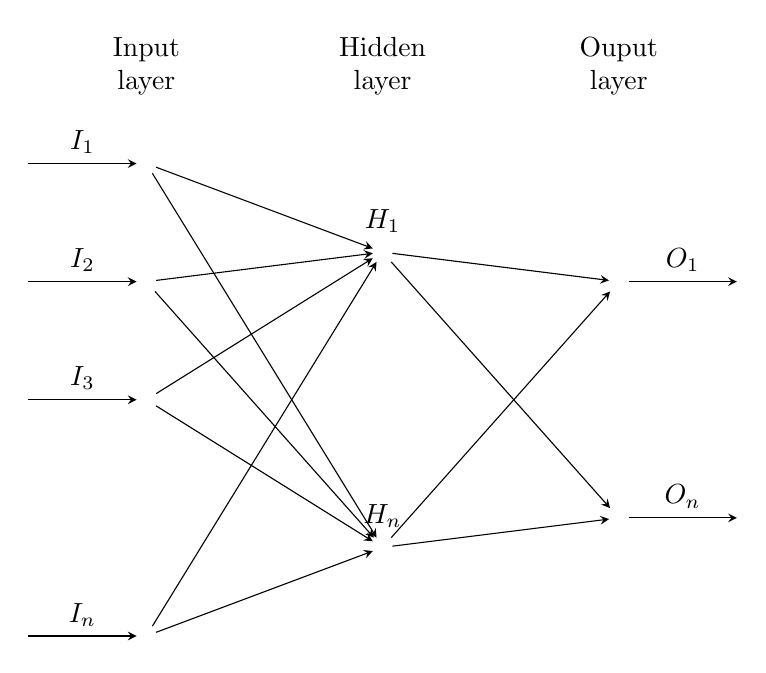
\begin{tikzpicture}[x=1.5cm, y=1.5cm, >=stealth]
	
	\foreach \m/\l [count=\y] in {1,2,3,missing,4}
	\node [every neuron/.try, neuron \m/.try] (input-\m) at (0,2.5-\y) {};
	
	\foreach \m [count=\y] in {1,missing,2}
	\node [every neuron/.try, neuron \m/.try ] (hidden-\m) at (2,2-\y*1.25) {};
	
	\foreach \m [count=\y] in {1,missing,2}
	\node [every neuron/.try, neuron \m/.try ] (output-\m) at (4,1.5-\y) {};
	
	\foreach \l [count=\i] in {1,2,3,n}
	\draw [<-] (input-\i) -- ++(-1,0)
	node [above, midway] {$I_\l$};
	
	\foreach \l [count=\i] in {1,n}
	\node [above] at (hidden-\i.north) {$H_\l$};
	
	\foreach \l [count=\i] in {1,n}
	\draw [->] (output-\i) -- ++(1,0)
	node [above, midway] {$O_\l$};
	
	\foreach \i in {1,...,4}
	\foreach \j in {1,...,2}
	\draw [->] (input-\i) -- (hidden-\j);
	
	\foreach \i in {1,...,2}
	\foreach \j in {1,...,2}
	\draw [->] (hidden-\i) -- (output-\j);
	
	\foreach \l [count=\x from 0] in {Input, Hidden, Ouput}
	\node [align=center, above] at (\x*2,2) {\l \\ layer};
	
	\end{tikzpicture}
\end{minipage}


\subsection{Acoustic Modelling using TDNNs.} 
%%% LaTeX2e class for student theses
%% sections/content.tex
%% 
%% Karlsruhe Institute of Technology
%% Institute for Program Structures and Data Organization
%% Chair for Software Design and Quality (SDQ)
%%
%% Dr.-Ing. Erik Burger
%% burger@kit.edu
%%
%% Version 1.3.2, 2017-08-01

\chapter{Design of a TDNN acoustic model}
\label{ch:tdnn_design}
Our approach for creating a robust TDNN acoustic model is to find a TDNN model that performs good on clean data first. Therefore, we had to make several design decisions. Most of the design decisions were justified by experiments, while some were taken from related work. This chapter summarizes the decisions made and the corresponding results. It should be noted that the experiments about robust acoustic modeling with TDNNs described in \cite{peddinti2015jhu} and \cite{peddinti2015reverberation} provided the main motivation for this work, therefore we based some of our parameters on their result.
\section{Training Data and System Setup}
All experiments in this work only concern the neural network part of our acoustic model, which is a HMM/TDNN hybrid. The speech recognition system itself, as well as all data, the HMM part of the acoustic model, the dictionary and the language model, are based upon the system described in \cite{nguyen20162016}. The system is built upon the Janus recognition toolkit \cite{finke1997karlsruhe}. We utilize a four-gram language model and the CMU Pronouncing Dictionary \cite{cmudict}, which uses 39 phones. The acoustic model uses quinphones and has 8156 different distributions, which means that the HMM part of our acoustic model has 8156 different states. \\ \\
The training and test dataset for the acoustic model consist of 468 hours of English speech from the TED-LIUM v2 \cite{rousseau2014enhancing}, Broadcast News \cite{graff19971996} and Quaero 2010-2012 datasets. From these 468~hours, 17~hours are randomly selected as test set, 451~hours are used for the training set. \\ \\
The development dataset, used for tuning the decoder parameters, consists of the english IWSLT 2013 evaluation dataset for the ASR track \cite{cettolo2013report}. This dataset consists of 3.9~hours of TED talks. The word error rates for all experiments in this chapter were measured on this development set. \\ \\ 
Each frame of samples in the datasets consists of 40~log-mel features which were normalized over the whole utterance to have mean zero and variance two. Each frame covers 32~milliseconds. The frame shift between successive frames is 10~milliseconds. The sampling rate of the audio data was 16~kHz. \\ \\
The neural network training was done using a custom framework, build on top of PyTorch \cite{paszke2017automatic}. Pytorch is a machine learning framework that supports GPU accelleration, parallelization along multiple systems and automatic differentiation. In the context of this work, several contributions were made to the PyTorch framework.  
\section{Neural Network Parameters}
This section focuses on parameters that are related to the neural network design. For all models in this section, the word error rate was estimated by using $l_p$ and $l_z$ that were tuned for each model separately. The priors were estimated by counting labels over the whole training set.
\subsection{Input Context}
The time input context of all our TDNN models is $(-13,9)$, which means the TDNN sees the current frame, thirteen frames in the past, and nine frames in the future. This parameter was taken from the smallest TDNN model described in \cite{peddinti2015reverberation}.
\subsection{Count and Width of Layers}
The count of layers and width of each layer is one of the most important design parameters for neural networks. As in \cite{peddinti2015reverberation}, all our models use the same amount of channels for each TDNN layer. Only the count of observed time frames changes with each layer. \\ \\
\begin{minipage}{\linewidth}
	\centering
	\begin{tabular}{@{\extracolsep{4pt}}lccccccccc@{}}
		\toprule
		Model:      & \multicolumn{4}{c}{Four Layer}       & \multicolumn{5}{c}{Five Layer}\\\cmidrule[1pt]{1-1}\cmidrule[1pt]{2-5}\cmidrule[1pt]{6-10}
		Layer       & 1 & 2 & 3 & 4    & 1 & 2 & 3 & 4 & 5 \\\cmidrule{2-5}\cmidrule{6-10}
		Kernel Size & 5 & 2 & 2 & 2    & 5 & 5 & 3 & 2 & 2 \\
		Stride      & 3 & 2 & 2 & 2    & 2 & 1 & 1 & 1 & 1 \\
		\bottomrule
	\end{tabular}
	\captionof{table}{Kernel size and stride parameters for the two different architectures}
	\label{tbl:tdnn_layer_design}
\end{minipage} \\ \\
We decided to test a four layer model with exactly the same parameters as the smallest model in \cite{peddinti2015reverberation}. This model also included a splicing layer after layer one. The splicing configuration was $(0, 1, 2, 3, 3, 4, 5, 6)$, relative to the previous layer. For the second model we tested, we decided to use larger kernels and one more layer. For this purpose, we removed the splicing layer and increased the layer count to five. Table \ref{tbl:tdnn_layer_design} gives the kernel size and stride over time for each layer in each architecture. For both models, we used an L2 pooling nonlinearity with group size of ten followed by a batch normalization layer after each TDNN layer.
\\
Figure \ref{fig:tdnn_layer_design} shows the word error rate for the two different architectures, given the count of channels. It can be seen that the four-layer architecture performed better than the five-layer architecture. We found the optimal count of channels  for the four-layer model to be 300. This contradicts \cite{peddinti2015reverberation}, where 400 channels were used. \\ \\
\begin{minipage}{\linewidth}
	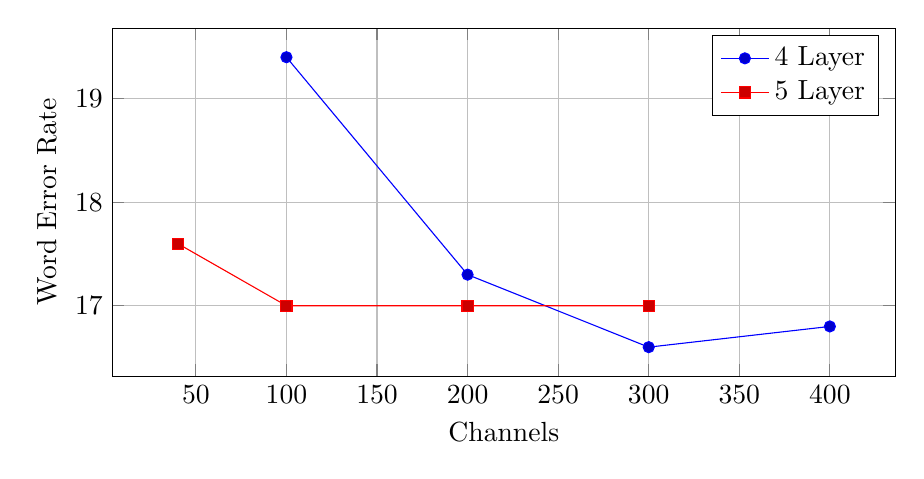
\begin{tikzpicture}
	\begin{axis}[ylabel=Word Error Rate, xlabel=Channels, height=6cm, 
	xticklabel style={name=T\ticknum},grid=major]
	\addplot coordinates {
		(100,19.4) %994
		(200,17.3) %999
		(300,16.6) %1009
		(400,16.8) %1010
	};
	\addlegendentry{4 Layer};
	\addplot coordinates {
		(40,17.6) %1040
		(100,17.0) %i3
		(200,17.0) %1039
		(300,17.0) %1036
	};
	\addlegendentry{5 Layer};
	\end{axis}
	\end{tikzpicture}
	\captionof{figure}{Word Error Rate for different choices of layer and channel count}
	\label{fig:tdnn_layer_design}
\end{minipage} 
\subsection{Nonlinearity}
\label{sec:tdnn_nonlin}
Following \cite{zhang2014improving}, we tested L2 pooling nonlinearity with group size if ten after each TDNN layer. Using the L2 norm can be problematic, as the gradient is not defined when all inputs in the pooling group are zero. The authors of \cite{zhang2014improving} propose to use a modified batch normalization layer after each LP-pooling layer, which solves the problem. We propose an alternate approach, which is setting the gradient to zero if all inputs become zero. Furthermore, we also tested max pooling as a possible nonlinearity. All experiments were conducted on the four-layer architecture described before. Figure \ref{fig:tdnn_nonlinearity} shows the results. \\ \\
\begin{minipage}{\linewidth}
	\centering
	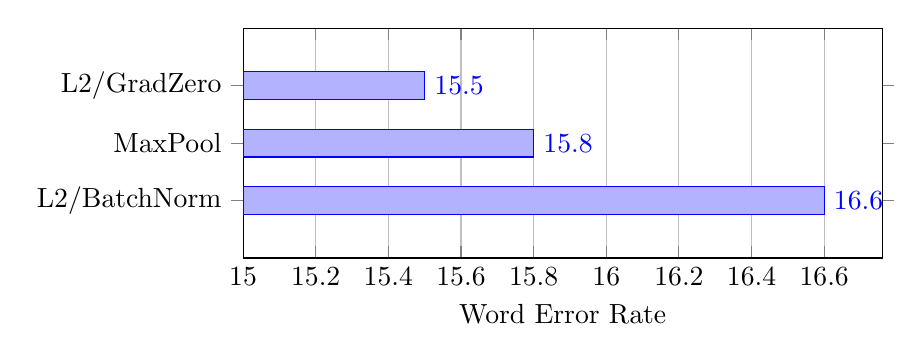
\begin{tikzpicture}
		\begin{axis}[
		xbar,xmajorgrids=true,
		width=0.8\linewidth,height=4.5cm, enlarge y limits=0.5,
		xmin=15,xlabel={Word Error Rate},
		symbolic y coords={L2/BatchNorm,MaxPool,L2/GradZero},
		ytick=data,nodes near coords, nodes near coords align={horizontal},
		]
		%1009, I24, I12
		% All with only l[/lz/mb tuning, no custom priors and no softmax
		\addplot coordinates {(15.5,L2/GradZero) (15.8,MaxPool) 
		(16.6,L2/BatchNorm)};
		\end{axis}
	\end{tikzpicture}
	\captionof{figure}{Word Error Rate for different choices of nonlinearities}
	\label{fig:tdnn_nonlinearity}
\end{minipage} \\ \\
In our case, the usage of L2 pooling with a modified gradient outperformed the other nonlinearities. It was not possible to compare L2 pooling without any modifications, as our training became unstable. 
\section{Training Setup}
This section is focused on the training setup for our acoustic model. Out setup is closely related to the setup described in \cite{nguyen20162016}. We essentially use the same speech recognition system, the same labels, as well as the same samples for training our acoustic model.
\subsection{Shuffling and Preparation of Dataset}
For our experiments, we benchmarked different shuffling strategies with a six-layer fully connected network. Shuffling of the whole dataset once before training, and shuffling of the whole dataset before each epoch. The results can be seen in figure \ref{fig:tdnn_shuffling}. \\ \\
\begin{minipage}{\linewidth}
	\centering
	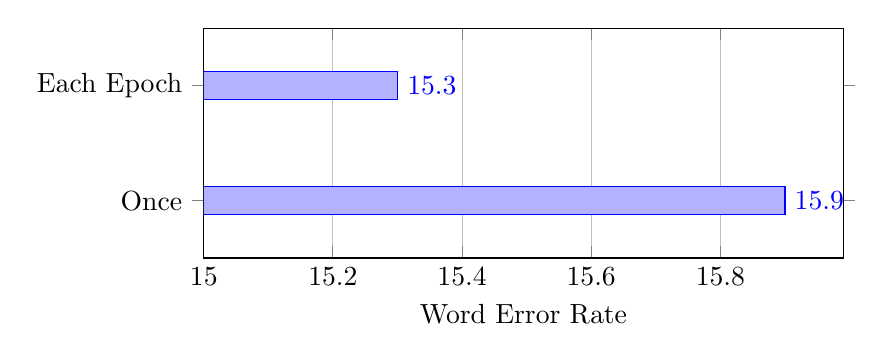
\begin{tikzpicture}
	\begin{axis}[
	xbar,xmajorgrids=true,
	width=0.8\linewidth,height=4.5cm, enlarge y limits=0.5,
	xmin=15,xlabel={Word Error Rate},
	symbolic y coords={Once,Each Epoch},
	ytick=data,nodes near coords, nodes near coords align={horizontal},
	]
	\addplot coordinates {(15.9,Once) (15.3,Each Epoch)};
	\end{axis}
	\end{tikzpicture}
	\captionof{figure}{Word Error Rate for different shuffling strategies}
	\label{fig:tdnn_shuffling}
\end{minipage} \\ \\
We can see that shuffling of the training dataset before each epoch decreased the word error rate. \\
\subsection{Learning Rate and Learning Rate Decay}
As in \cite{nguyen20162016}, we utilize the newbob learning rate scheduler for training for stochastic gradient descend, with an initial learning rate of $0.08$ and a momentum of $5$. The SGD variant used is the introduced in section \ref{sec:momentum}, as this was also used in \cite{nguyen20162016}\footnote{This SGD variant is not equal to the default SGD variant implemented in pytorch.}. Figure \ref{fig:newbob_wer} shows the word error rate per epoch when using newbob. It can be seen that there were almost no improvements during epoch four, but the word error rate improved as soon as the decaying started after epoch four. Figure \ref{fig:newbob_fer} shows the frame error rate per epoch for the same training run. It can be seen that exponential decay reduces the frame error rate significantly. The model used for this experiment was the four layer TDNN introduced in the previous section.
\\ \\
\begin{minipage}{\linewidth}
	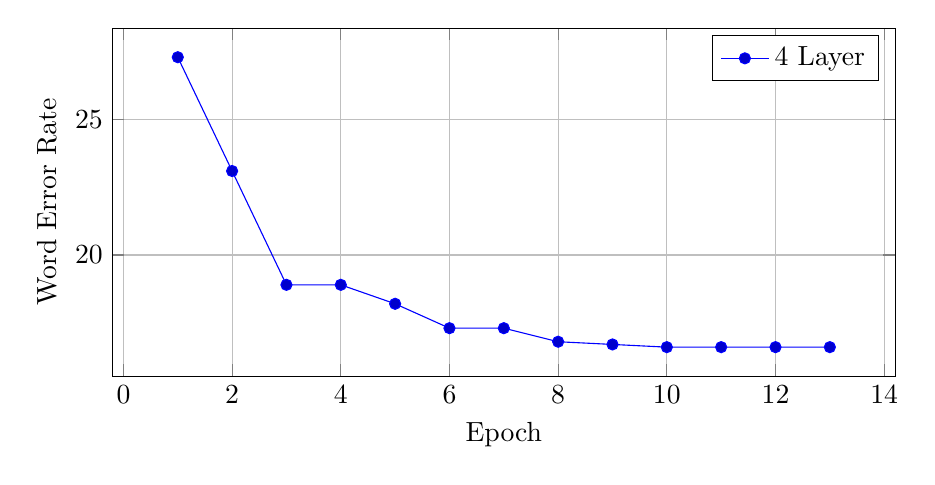
\begin{tikzpicture}
	\begin{axis}[ylabel=Word Error Rate, xlabel=Epoch, height=6cm, 
	xticklabel style={name=T\ticknum},grid=major]
	% I12
	\addplot coordinates {
		(1,27.3)
		(2,23.1)
		(3,18.9)
		(4,18.9)
		(5,18.2)
		(6,17.3)
		(7,17.3)
		(8,16.8)		
		(9,16.7)
		(10,16.6)
		(11,16.6)
		(12,16.6)
		(13,16.6)
	};
	\addlegendentry{4 Layer};
	\end{axis}
	\end{tikzpicture}
	\captionof{figure}{Word Error Rate per Epoch when using newbob training. The exponential decaying of the learning rate started after epoch four.}
	\label{fig:newbob_wer}
\end{minipage}
 \\ \\
\begin{minipage}{\linewidth}
	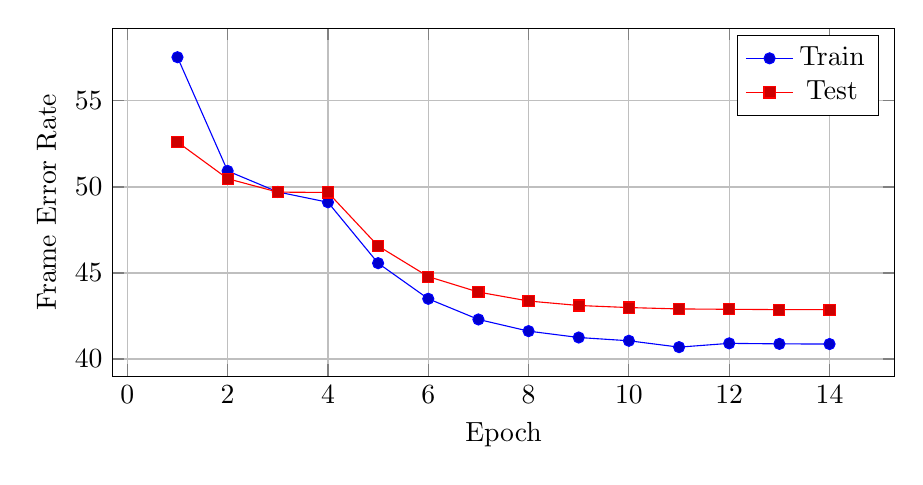
\begin{tikzpicture}
	\begin{axis}[ylabel=Frame Error Rate, xlabel=Epoch, height=6cm, 
	xticklabel style={name=T\ticknum},grid=major]
	%I12
	\addplot coordinates {
		(1,57.54)
		(2,50.93)
		(3,49.71)
		(4,49.11)
		(5,45.57)
		(6,43.50)
		(7,42.30)
		(8,41.62)		
		(9,41.25)
		(10,41.06)
		(11,40.69)
		(12,40.91)
		(13,40.88)
		(14,40.87)
	};
	\addlegendentry{Train};
	\addplot coordinates {
		(1,52.61)
		(2,50.48)
		(3,49.70)
		(4,49.68)
		(5,46.57)
		(6,44.79)
		(7,43.89)
		(8,43.37)		
		(9,43.11)
		(10,42.99)
		(11,42.91)
		(12,42.89)
		(13,42.87)
		(14,42.87)
	};
	\addlegendentry{Test};
	\end{axis}
	\end{tikzpicture}
	\captionof{figure}{Frame Error Rate per Epoch when using newbob training. The exponential decaying of the learning rate started after epoch four.}
	\label{fig:newbob_fer}
\end{minipage}
\subsection{MMIE Training}
Since the experiments described in \cite{peddinti2015jhu} show improvement when sMBR discriminative training is used, we attempted to use discriminative based training as well. Our implementation used maximum mutual information estimation, as described in section \ref{sec:mmie}. We picked this training variant as a first step, since it is easier to implement than any variant of overall risk criterion estimation. Both approaches should show some improvement over cross entropy loss on frame level, according to several bodies of work \cite{povey2005discriminative} \cite{ghoshal2013sequence}. \\ \\
For MMIE training, we pre-trained a four layer TDNN acoustic model with frame-based cross entropy loss for a single epoch. Then, we started MMIE training on a per-utterance basis. For this purpose, we wrote a module that enabled interoperability between the Janus recognition toolkit and PyTorch. The training was done on multiple machines with a total of 256 processors, the gradients were averaged before each SGD step. \\ \\
While our experiments consistently showed high improvements in terms of frame error rate, the word error rate increased significantly: The model reached a WER of $17.6$ using cross entropy loss, but only a WER $25.6$ was reached after the MMIE training finished the first epoch. This effect was also described in more practically oriented literature \cite{su2013error} for MMIE without any further modifications. 

\begin{minipage}{\linewidth}
	\begin{minipage}{0.5\linewidth}
	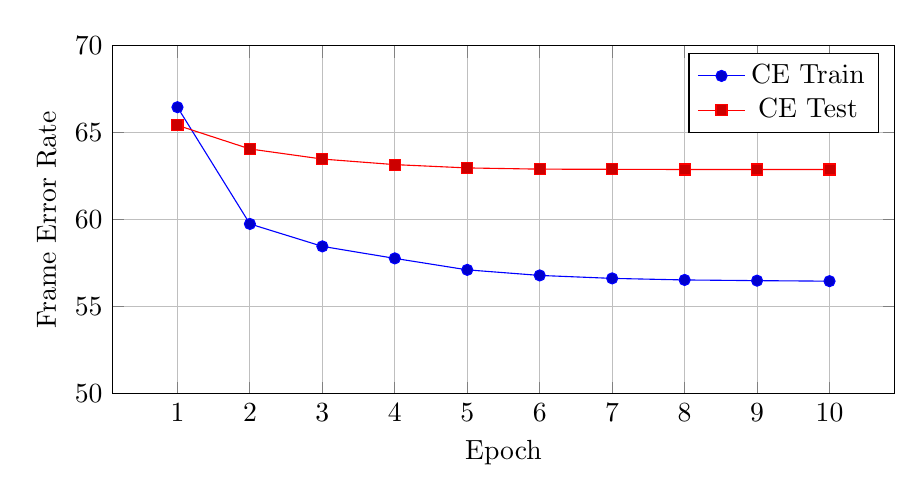
\begin{tikzpicture}
	\begin{axis}[ylabel=Frame Error Rate, xlabel=Epoch, height=6cm, 
	ymin=50, ymax=70,
	xticklabel style={name=T\ticknum},grid=major]
	%1040
	\addplot coordinates {
		(1,66.47)
		(2,59.76)
		(3,58.47)
		(4,57.78)
		(5,57.12)
		(6,56.80)
		(7,56.63)
		(8,56.54)		
		(9,56.50)
		(10,56.47)
	};
	\addlegendentry{CE Train};
	\addplot coordinates {
		(1,65.43)
		(2,64.07)
		(3,63.49)
		(4,63.17)
		(5,62.98)
		(6,62.91)
		(7,62.90)
		(8,62.89)		
		(9,62.89)
		(10,62.89)
	};
	\addlegendentry{CE Test};
	\end{axis}
	\end{tikzpicture}
\end{minipage}
\hfill
\begin{minipage}{0.5\linewidth}
	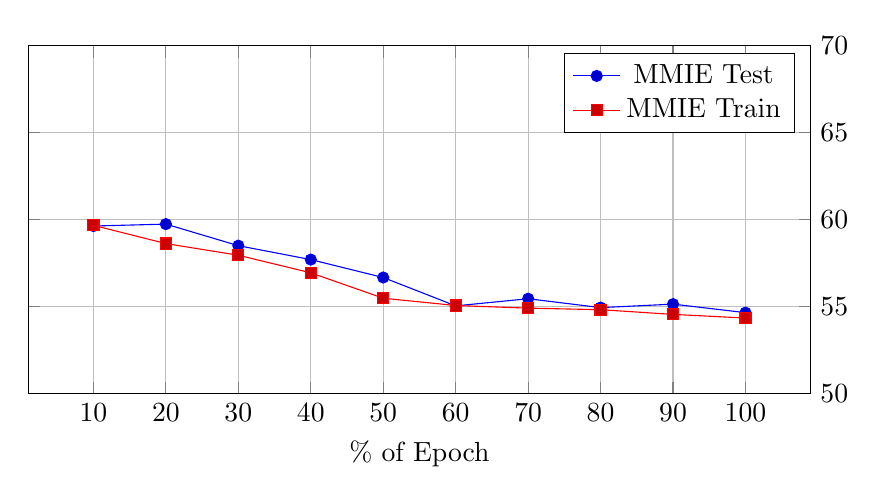
\begin{tikzpicture}
	\begin{axis}[xlabel=\% of Epoch, height=6cm, 
	 ylabel near ticks, yticklabel pos=right,
	ymin=50, ymax=70,
	xticklabel style={name=T\ticknum},grid=major]
	%1040 SMBR 24
	\addplot coordinates {
		(10,59.64)
		(20,59.75)
		(30,58.51)
		(40,57.71)
		(50,56.68)
		(60,55.05)
		(70,55.46)
		(80,54.95)		
		(90,55.15)
		(100,54.66)
	};
	\addlegendentry{MMIE Test};
	\addplot coordinates {
		(10,59.68)
		(20,58.631)
		(30,57.96)
		(40,56.95)
		(50,55.49)
		(60,55.07)
		(70,54.92)
		(80,54.83)		
		(90,54.56)
		(100,54.35)
	};
	\addlegendentry{MMIE Train};
	\end{axis}
	\end{tikzpicture}
\end{minipage}
	\captionof{figure}{Frame Error Rate per Epoch when using cross entropy loss, as well as Frame Error Rate over a single epoch when using MMIE on a TDNN}
	\label{fig:mmie_fer}
\end{minipage} \\ \\
Detailed results regarding the frame error rate are shown in figure \ref{fig:mmie_fer}. It can be seen that the MMIE training converged significantly faster than cross entropy training. Also, the error on the test data set is significantly closer to the error on the training data set. 
\iffalse
% This is the training for a Fully Connected net with ReLU, which diverged. There are examples in the litherature which did NOT diverge. 
\begin{minipage}{\linewidth}
	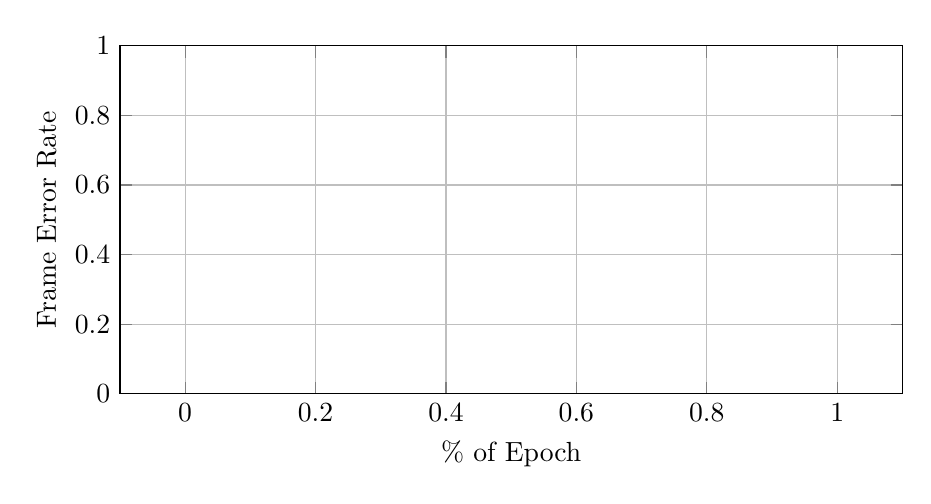
\begin{tikzpicture}
	\begin{axis}[ylabel=Frame Error Rate, xlabel=\% of Epoch, height=6cm, 
	ymin=50, ymax=70,
	xticklabel style={name=T\ticknum},grid=major]
	%1040
	\addplot coordinates {
		(10,75.2618)
		(20,75.2638)
		(30,75.2839)
		(40,76.25)
		(50,76.99539216)
		(60,87.03598039)
		(70,83.21137255)
		(80, 84.23852941)
	};
	\addlegendentry{MMIE Train};
	\end{axis}
	\end{tikzpicture}
	\label{fig:mmie_fer_fc}
\end{minipage}
\fi
\\ These results were achieved using the four-layer TDNN model. Caution has to be taken when interpreting the results: While the amount of data in both test data sets is the same, they are not equal as training and testing for MMIE happens on per-utterance basis, while the test and training sets for the cross entropy loss based training were created on per-frame basis. \\ \\
Although the results regarding frame error rate look interesting, we did not pursue this approach any further, due to the resulting high word-error rates and the numerous details one has to consider for working MMIE training on neural networks \cite{su2013error}.

\section{Decoding Parameters}
Tuning decoding parameters is important for good achieving a high accuracy on word level. The decoding parameters are not directly related to the acoustic model, but rather the decoding process. Different acoustic models might still require different decoding parameters for best performance. 
\subsection{Acoustic Model Scaling and Length Penalty}
Our experiments have shown that the $l_p$ and $l_z$ parameters are depending on each other. Therefore we can not optimize them separately. We choose to perform a grid search over a reasonable parameter space. \\ \\
\begin{minipage}{\linewidth}
\centering
\begin{tikzpicture}
\begin{axis}[grid=both,zlabel=Word Error Rate,xlabel=$l_p$,ylabel=$l_z$,width=0.7\linewidth]
	\addplot3[surf,mesh/cols=10,z buffer=sort] file {data/lp_lz_i12};
\end{axis}
\end{tikzpicture}
\captionof{figure}{Illustrative example of the word error rate for different $l_p$ and $l_z$ parameters for a four-layer TDNN}
\label{fig:lp_lz}
\end{minipage}
\\ \\
An example impact of the $l_p$ and $l_z$ for two different models are illustrated in figure \ref{fig:lp_lz}. Our experiments have shown that the optimal parameters are similar for each of the models we tested. It is still advisable to fine tune the parameters for each model. Taking the initial values for the grid search from an similar model usually leads to good results.
\subsection{Master Beam}
We tested several architectures with different master beams. Master beams between four and six appeared to work best, but we did not find any pattern that correlated with the network architecture. This indicates that the optimal master beam depends on several factors, not just on the architecture of the neural network model itself. 
\subsection{Neural Network Priors}
\label{sec:tdnn_prior}
As described in section \ref{sec:ce_loss}, it is important to scale the posteriors generated by the neural network with priors. We tested two different approaches of generating the priors: Generating them from the complete test dataset and also generating them from the output of a trained model. In the second case, we selected thirty minutes of speech data randomly from our dataset, computed the neural network output on it, and counted the occurrence of each label in the output. \\ \\
\begin{minipage}{\linewidth}
	\centering
	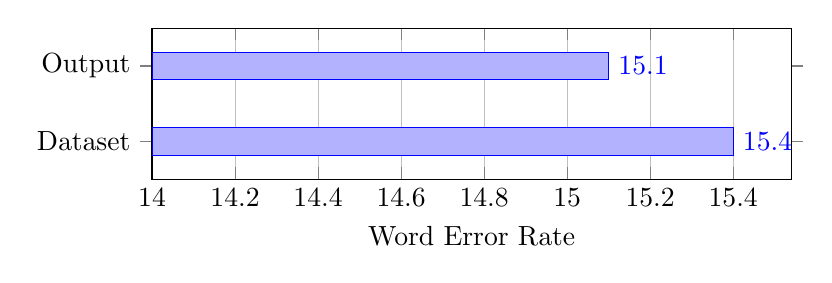
\begin{tikzpicture}
	\begin{axis}[
	xbar,xmajorgrids=true,
	width=0.8\linewidth,height=3.5cm, enlarge y limits=0.5,
	xmin=14,xlabel={Word Error Rate},
	symbolic y coords={Dataset,Output},
	ytick=data,nodes near coords, nodes near coords align={horizontal},
	]
	\addplot coordinates {(15.4,Dataset) (15.1,Output)};
	\end{axis}
	\end{tikzpicture}
	\captionof{figure}{Word Error Rate for priors estimated from the dataset and the model output}
	\label{fig:wer_priors}
\end{minipage} 
\\
As illustrated in figure \ref{fig:wer_priors}, calculating the priors from the the output of the model decreased the word error rate significantly. These experiments were done on the four-layered TDNN model. 
\subsection{Softmax Smoothing}
We also tested the impact of softmax smoothing on the neural network output. The motivation is that a beam search through a hidden Markov model does not work very well when the acoustic model is overconfident regarding certain states. Figure \ref{fig:softmax_fer} shows that softmax smoothing decreased the word error rate for our four-layer TDNN model. \\ \\
\begin{minipage}{\linewidth}
	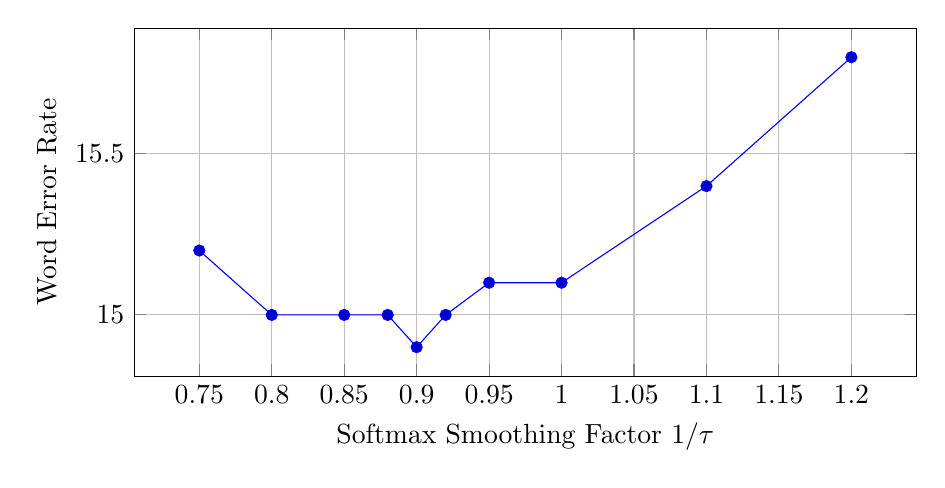
\begin{tikzpicture}
	\begin{axis}[ylabel=Word Error Rate, xlabel=Softmax Smoothing Factor $1/\tau$, height=6cm, 
	xticklabel style={name=T\ticknum},grid=major]
	%I12
	\addplot coordinates {
		(0.75,15.2)
		(0.8,15)
		(0.85,15)
		(0.88,15)
		(0.9,14.9)
		(0.92,15)
		(0.95,15.1)
		(1,15.1)
		(1.1,15.4)
		(1.2,15.8)
	};
	\end{axis}
	\end{tikzpicture}
	\captionof{figure}{Word Error Rate per softmax adjustment $1/\tau$ for a four-layer TDNN model}
	\label{fig:softmax_fer}
\end{minipage} \\ \\


\iffalse
\label{ch:approach}
This chapter describes our approach for acoustic modelling using TDNNs on a high level. 
We will also give a brief overview over unknown hyperparemters and design decisions,
as well as a coarse overview over the structure of our implementation. 

\chapter{Experiment Setup}
\label{ch:experiment_setup}
This chapter should describe the detailed preleminaries and hyperparemters of our training and evaluation setup:
\begin{itemize}
    \item which data, and which preprocessing was used
    \item how was the data reverbed
    \item which learning rate schedulers, optimizers, loss functions were used
    \item which mechanisms were used to make the training faster and scalable
\end{itemize}
\fi
%%% LaTeX2e class for student theses
%% sections/evaluation.tex
%% 
%% Karlsruhe Institute of Technology
%% Institute for Program Structures and Data Organization
%% Chair for Software Design and Quality (SDQ)
%%
%% Dr.-Ing. Erik Burger
%% burger@kit.edu
%%
%% Version 1.3.2, 2017-08-01

\chapter{Evaluation on Reverberated Data}
\label{ch:results}
This section contains the final evaluation. It describes how different models performed on reverberated data.
\section{Neural Network Models}
We compare the four-layer TDNN model with a fully connected baseline model that was also used in \cite{nguyen20162016}. 
\subsection{TDNN Model}
The TDNN model, which can be seen in figure \ref{fig:final_tdnn} is based on the results found in chapter \ref{ch:tdnn_design}. \\ 
\begin{minipage}{\linewidth}
	\vspace{5mm}
	\begin{tikzpicture}[x=1.8cm, y=1.5cm]
	% Input layer
	\node[text width=3cm] at (-1,0) {Input ($23*40$)};
	\foreach \m in {2,3,...,22}
	\node [tdnn neuron] (input-\m) at (\m*0.25,0) {};
	
	\node [tdnn neuron, label=below:$x_{t - 13}$] (input-1) at (1*0.25,0) {};
	\node [tdnn neuron, label=below:$x_{t + 9}$] (input-23) at (23*0.25,0) {};
	
	% TDNN 1
	\node[text width=3cm] at (-1,0.5) {TDNN/LP 1};
	\node[text width=3cm] at (-1,1) {Hidden ($7*300$)};
	\foreach \m [count=\y] in {1,2,...,7}
	\node [tdnn neuron] (hidden-1-\m) at (\y*0.25*3,1) {};
	
	% Splice
	\node[text width=3cm] at (-1,1.5) {Splice};
	\node[text width=3cm] at (-1,2) {Hidden ($8*300$)};
	\foreach \m [count=\y] in {1,2,...,8}
	\node [tdnn neuron] (hidden-2-\m) at (\y*0.25*3 - 0.40,2) {};
	
	% TDNN 2
	\node[text width=3cm] at (-1,2.5) {TDNN/LP 2};
	\node[text width=3cm] at (-1,3) {Hidden ($4*300$)};
	\foreach \m [count=\y] in {1,2,...,4}
	\node [tdnn neuron] (hidden-3-\m) at (\y*0.25*6 - 0.80,3) {};
	
	% TDNN 3
	\node[text width=3cm] at (-1,3.5) {TDNN/LP 2};
	\node[text width=3cm] at (-1,4) {Hidden ($2*300$)};
	\foreach \m [count=\y] in {1,2}
	\node [tdnn neuron] (hidden-4-\m) at (\y*0.25*12 - 1.60,4) {};
	
	% TDNN 4
	\node[text width=3cm] at (-1,4.5) {TDNN/LP 2};
	\node[text width=3cm] at (-1,5) {Hidden ($1*400$)};
	\node [tdnn neuron] (hidden-5) at (1*0.25 + 11 * 0.25,5) {};
	
	% Classifier
	\node[text width=3cm] at (-1,5.5) {Linear/Softmax};
	\node[text width=3cm] at (-1,6) {Output ($1*8156$)};
	\node [tdnn neuron, label=above:$y_{t}$] (classify-1) at (1*0.25 + 11 * 0.25,6) {};
	
	% Edges
	%L1 Edges
	\foreach \m [
	evaluate=\m as \nstart using int(((\m - 1) * 3) + 1),
	evaluate=\m as \nstep using int(((\m - 1) * 3) + 2),
	evaluate=\m as \nend using int(((\m - 1)* 3) + 5)] in {1,2,...,7}
	\foreach \i in {\nstart,\nstep,...,\nend}
	\draw (input-\i.north) -- (hidden-1-\m);  
	
	%Splice Edge
	\draw (hidden-1-1.north) -- (hidden-2-1.south);  
	\draw (hidden-1-2.north) -- (hidden-2-2.south);
	\draw (hidden-1-3.north) -- (hidden-2-3.south);
	\draw (hidden-1-4.north) -- (hidden-2-4.south);
	\draw (hidden-1-4.north) -- (hidden-2-5.south);
	\draw (hidden-1-5.north) -- (hidden-2-6.south);
	\draw (hidden-1-6.north) -- (hidden-2-7.south);
	\draw (hidden-1-7.north) -- (hidden-2-8.south);
	
	% Edges
	%L2 Edges
	\foreach \m [
	evaluate=\m as \na using int(((\m - 1) * 2) + 1),
	evaluate=\m as \nb using int(((\m - 1) * 2) + 2)] in {1,2,...,4} {
		\draw (hidden-2-\na.north) -- (hidden-3-\m);
		\draw (hidden-2-\nb.north) -- (hidden-3-\m);
	}
	
	%Edges
	%L3 Edges
	\draw (hidden-3-1.north) -- (hidden-4-1);
	\draw (hidden-3-2.north) -- (hidden-4-1);
	\draw (hidden-3-3.north) -- (hidden-4-2);
	\draw (hidden-3-4.north) -- (hidden-4-2);
	
	%L4 edges
	\draw (hidden-4-1) -- (hidden-5);
	\draw (hidden-4-2) -- (hidden-5);

	% Classify Edges
	\draw (hidden-5) -- (classify-1);
	
	\end{tikzpicture}
	\captionof{figure}{Illustration of the final TDNN model in the time domain}
	\label{fig:final_tdnn}
	\vspace{5mm}
\end{minipage}\\ \\
It consists of four TDNN layers and one linear layer at the end, followed by a softmax nonlinearity. After each TDNN layer, a L2 pooling nonlinearity with zeroing of unstable gradients and a pool size of ten is used. A splicing layer with the splicing configuration $(0, 1, 2, 3, 3, 4, 5, 6)$ was used after the first TDNN layer. The exact configuration of kernel sizes and strides can be found in table \ref{tbl:tdnn_layer_design}. The output of each TDNN layer had 3000 channels, the output of each pooling layer 300 channels. The input context consisted was $(-13, 9)$. The count of channels, the modified L2 pooling gradient and the omission of batch normalization was the main difference to the architecture described in \cite{peddinti2015reverberation} and \cite{peddinti2015jhu}. 
\subsection{Fully Connected Baseline Model}
We compare the results of our TDNN with a fully connected network that achieved comparable performance on an reverberated training set. The model consists of six linear layers with a width of 1600, followed by ReLU nonlinearities. The output layer is a linear layer followed by a Softmax nonlinearity. We tested input contexts of $(-13, 9)$ as well as $(-5, 5)$.
\section{Training Setup}
We used the same training set as described in chapter \ref{ch:tdnn_design} as well as a reverberated version of the training set. As in chapter \ref{ch:tdnn_design}, we used a SGD variant with newbob learning rate scheduling and momentum. The loss function was frame based cross entropy loss. The input features at each time frame were 40 log-mel coefficients as in \cite{nguyen20162016}. Our input features were mean normalized over the whole utterance with a mean of zero and a variance of two. This is different from the unnormalized 140 dimensional input vector used by \cite{peddinti2015reverberation} in \cite{peddinti2015jhu} for their TDNN model.
\section{Data Augmentation}
For training and evaluating acoustic models that are robust on reverberated data, we trained them on data that was reverberated as well. For this purpose, we used a collection of recorded room impulse responses to augment our data set. This follows the theoretical insight given in section \ref{sec:reverberation}: For each audio sequence in our data set, we pick a random room impulse response and convolute the two signals to from an augmented signal. \\ \\
The room impulse responses we used are similar as in \cite{ritter2016training}. However we did only use the RWCP \cite{nakamura2000acoustical}, OMNI \cite{stewart2010database} and ACE \cite{eaton2015ace} datasets. The AIR dataset  \cite{jeub2009binaural} was not used, since the amplitude in the different recordings in the dataset change significantly.
Evaluating the effects of different signal amplitudes was not a goal of this work, as we can assume that the audio frontend used will always provide a reasonable gain. We therefore normalized the room impulse responses very carefully before performing the convolution based on their signal energy. For the ACE dataset, we found that the energy direct transmission path was very low compared to the noise. In this case, we amplified the direct transmission path to generate a meaningful result.
Illustration \ref{fig:air_spectrogram} shows an audio sample that was reverberated with this method. 
\section{Evaluation Results}
We test the four-layer TDNN model with the input context $(-13, 9)$, as well as the fully connected (\textit{FC}) model with the input contexts $(-13, 9)$ and $(-5, 5)$. To do so, we train each model on the clean training set as described in chapter \ref{ch:tdnn_design}. We separately tune each model on a combination on the clean and reverberated training set, with a total length of 902~hours. Then, we tune the $l_p$, $l_z$, master beam and softmax temperature parameters using the development set mentioned in chapter \ref{ch:tdnn_design}. The development set was not augmented. \\ \\ Since was impossible to fit the combined 902~hour dataset entirely into memory, and loading from disk was very slow with the large input context of $(-13, 9)$, we reduced the precision of the training dataset to 16~bits for all experiments in this section. We validated this approach by also running several experiments different on the clean dataset with the original precision. The differences in terms of FER were below 0.1\% where sometimes the model trained on high precision and sometimes a model low precision was better. In terms of WER we did not observe any difference on the development set. \\ \\
For this evaluation we use the \textit{tst2014} dataset, which was the evaluation dataset for the IWSLT 2014 conference \cite{cettolo2014report}. Similar to our development dataset, the evaluation dataset also consists of TED talks with a total length of 2.1~hours. \\ \\
The TDNN model, which has 4.2~million parameters, trained for 14~epochs, where each epoch took 9.3~hours on the combined dataset, on a single GTX~1080~Ti~GPU. On the clean dataset, a single training epoch took 4.2~hours. The fully connected models with short and long input contexts had 13.2~million and 13.6~million parameters respectively. They trained for 12 and 11 epochs, where each epoch took 1.3~hours on the clean dataset and 2.3~hours on the combined dataset. 
\\ \\
The results of our evaluation can be seen in figure \ref{fig:final_validation}. For models trained on clean data, the word error rate on the reverberated development set is high. It can be seen that models with larger input context performed better on unseen reverberated data. On the clean validation set, all models performed similar. \\ \\
\begin{minipage}{\linewidth}
\begin{minipage}{\linewidth}
\centering
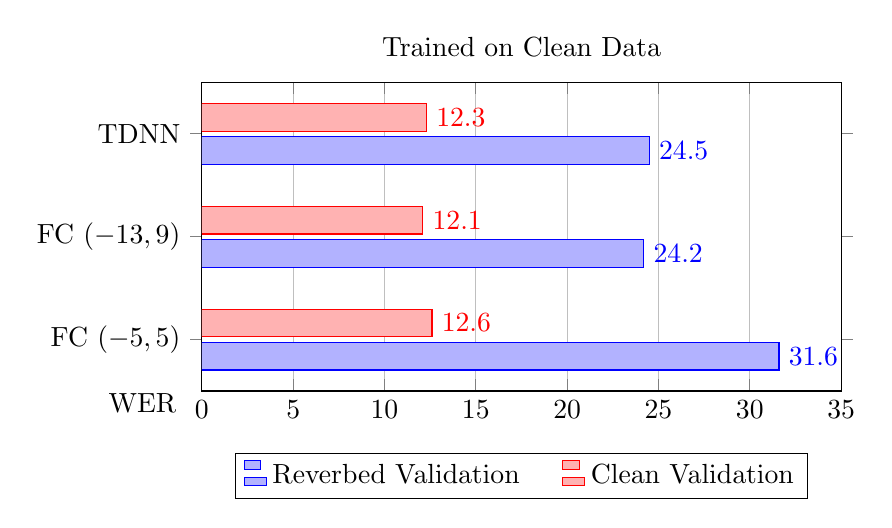
\begin{tikzpicture}
\begin{axis}[
title=Trained on Clean Data,
xbar,xmajorgrids=true,
width=0.8\linewidth,height=5.5cm, enlarge y limits=0.25,
xmin=0,xmax=35,xlabel={WER},xlabel style={
	at={(ticklabel cs:0)},
	anchor=north east,
	yshift=0.56 cm, xshift=-0.2cm
},
symbolic y coords={FC \text{$(-5,5)$}, FC \text{$(-13,9)$}, TDNN},
ytick=data,nodes near coords, nodes near coords align={horizontal},
legend style={at={(0.5,-0.2)},
	anchor=north,legend columns=2}
]
\addplot coordinates {(31.6,FC \text{$(-5,5)$}) (24.2,FC \text{$(-13,9)$}) (24.5,TDNN)};
\addlegendentry{Reverbed Validation \quad \quad}
\addplot coordinates {(12.6,FC \text{$(-5,5)$}) (12.1,FC \text{$(-13,9)$}) (12.3,TDNN)};
\addlegendentry{Clean Validation}
\end{axis}
\end{tikzpicture}
\end{minipage}
\\ \\ \\ 
\begin{minipage}{\linewidth}
\centering
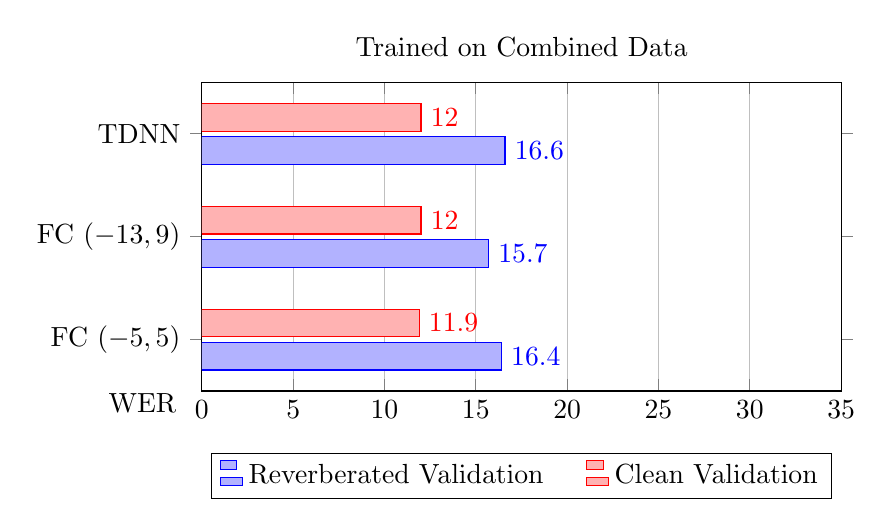
\begin{tikzpicture}
	\begin{axis}[
	title=Trained on Combined Data,
	xbar,xmajorgrids=true,
	width=0.8\linewidth,height=5.5cm, enlarge y limits=0.25,
	xmin=0,xmax=35,xlabel={WER}, xlabel style={
       at={(ticklabel cs:0)},
	   anchor=north east,
	   yshift=0.56 cm, xshift=-0.2cm
	},
	symbolic y coords={FC \text{$(-5,5)$}, FC \text{$(-13,9)$}, TDNN},
	ytick=data,nodes near coords, nodes near coords align={horizontal},
	legend style={at={(0.5,-0.2)},
		anchor=north,legend columns=2}
	]
	\addplot coordinates {(16.4,FC \text{$(-5,5)$}) (15.7,FC \text{$(-13,9)$}) (16.6,TDNN)};
	\addlegendentry{Reverberated Validation \quad \quad}
	\addplot coordinates {(11.9,FC \text{$(-5,5)$}) (12,FC \text{$(-13,9)$}) (12,TDNN)};
	\addlegendentry{Clean Validation}
	\end{axis}
	\end{tikzpicture}
	\captionof{figure}{Word Error Rate on the clean and reverberated validation dataset for models trained on clean and combined training data, respectively}
	\label{fig:final_validation}
\end{minipage} 
\end{minipage} 
\\ \\ \\
For models trained on reverberated data, the performance on reverberated validation is similar data for all three models. The same holds for clean validation data. The fully connected model with a large input context outperformed the other models on the reverberated validation set by a small margin. All models performed slightly better on clean validation data than the same model trained on clean data only, where the difference was most significant for the fully connected model with short input context. \\ \\
From this observations we conclude that data augmentation can be sufficient for improving acoustic model performance for reverberated audio. A larger input context can improve the robustness of the acoustic model in some cases. 
\iffalse
TODO: Describe how we generated reverbed data
TODO: Describe how we tested on reverbed data
TODO: Describe final architecture and results

This chapter should summarize and interpret the results. It should give a clear insight
about which methods did decrease the FER and WER on reverbed and unreverbed data, respectivley.
\fi
%%% LaTeX2e class for student theses
%% sections/conclusion.tex
%% 
%% Karlsruhe Institute of Technology
%% Institute for Program Structures and Data Organization
%% Chair for Software Design and Quality (SDQ)
%%
%% Dr.-Ing. Erik Burger
%% burger@kit.edu
%%
%% Version 1.3.2, 2017-08-01

\chapter{Conclusion}
\label{ch:Conclusion}
During our evaluation in chapter \ref{ch:results} we found that our TDNN model did not yield a significant improvement over a fully connected model when trained on reverberated data. We also found that a fully connected model with the same input context was capable of slightly outperforming our TDNN model on the reverberated data validation set. This results are difficult to generalize to TDNNs as a whole for the following reasons: 
\begin{itemize}
	\item In chapter \ref{ch:tdnn_design}, we tuned our TDNN on clean data, with the assumption that a TDNN model that performs well on clean data also performs well on reverberated data. 
	\item The room impulse response normalization given in \ref{ch:results} might have been too aggressive, thus negating the advantage of TDNNs. In general, it is hard to measure the comprehensibleness of reverberated audio objectively.  
	\item In literature \cite{peddinti2015jhu} \cite{peddinti2015reverberation}, sMBR training criteria are used for TDNN acoustic model training. It might be worth to investigate this training procedure more closely.  
\end{itemize}
While the question whether TDNNs or fully connected networks are better for this specific problem is still unanswered, we provide several interesting insights that can improve speech recognition systems:
\begin{itemize}
	\item The modified L2 pooling nonlinearity introduced in section \ref{sec:tdnn_nonlin} performed better than L2 pooling combined with normalization.
	\item Augmented data can be used to boost the performance of acoustic models, even when only clean audio is of concern, as shown in chapter \ref{ch:results}.
	\item The calculation of priors from the network output, as shown in section \ref{sec:tdnn_prior}, given a randomly sampled subset of the training data, was shown to outperform priors which were calculated from the training data set. 
\end{itemize}
Overall, we were able to show that acoustic models can be made robust against reverberation, if they are trained using reverberated data as well.

%% --------------------
%% |   Bibliography   |
%% --------------------

%% Add entry to the table of contents for the bibliography
\printbibliography[heading=bibintoc]

%% ----------------
%% |   Appendix   |
%% ----------------
\appendix
%% LaTeX2e class for student theses
%% sections/apendix.tex
%% 
%% Karlsruhe Institute of Technology
%% Institute for Program Structures and Data Organization
%% Chair for Software Design and Quality (SDQ)
%%
%% Dr.-Ing. Erik Burger
%% burger@kit.edu
%%
%% Version 1.3.2, 2017-08-01


\chapter{Appendix}
\label{ch:appendix}
The appendix will contain information that might be useful for readers but 
does not fit anywhere else:
\begin{itemize}
  \item Practical pitfalls during training
  \item Implementation details
  \item If applicable, raw result data
\end{itemize}

\end{document}
